\chapter{Stochastic Interventional Mediation Effects}

Causal mediation analysis has historically been limited in two important ways:
(i) a focus has traditionally been placed on binary exposures and static
interventions, and (ii) direct and indirect effect decompositions have been
pursued that are only identifiable in the absence of intermediate confounders
affected by exposure. We present a theoretical study of an (in)direct effect
decomposition of the population intervention effect, defined by stochastic
interventions jointly applied to the exposure and mediators. In contrast to
existing proposals, our causal effects can be evaluated regardless of whether
a exposure is categorical or continuous and remain well-defined even in the
presence of intermediate confounders affected by exposure. Our (in)direct
effects are identifiable without a restrictive assumption on cross-world
counterfactual independencies, allowing for substantive conclusions drawn from
them to be validated in randomized controlled trials. Beyond the novel effects
introduced, we provide a careful study of nonparametric efficiency theory
relevant for the construction of flexible, multiply robust estimators of our
(in)direct effects, while avoiding undue restrictions induced by assuming
parametric models of nuisance parameter functionals. To complement our
nonparametric estimation strategy, we introduce inferential techniques for
constructing confidence intervals and hypothesis tests, and discuss open source
software, the \texttt{medshift} \texttt{R} package, implementing the proposed
methodology. Application of our (in)direct effects and their nonparametric
estimators is illustrated using data from a comparative effectiveness trial
examining the direct and indirect effects of pharmacological therapeutics on
relapse to opioid use disorder.

%%%%%%%%%%%%%%%%%%%%%%%%%%%%%%%%%%%%%%%%%%%%%%%%%%%%%%%%%%%%%%%%%%%%%%%%%%%%%%%
\section{Introduction}\label{sec:intro}
%%%%%%%%%%%%%%%%%%%%%%%%%%%%%%%%%%%%%%%%%%%%%%%%%%%%%%%%%%%%%%%%%%%%%%%%%%%%%%%

In myriad applications, one is often interested in the effect of an exposure on
an outcome only through a particular pathway between the two. Indeed, efforts in
defining and identifying such \textit{path-specific} effects have come to
constitute a rich history in not only philosophy but also in the sciences of
statistics, causal inference, epidemiology, economics, and psychology. In each
of these disciplines, as well as in many others among the biomedical and social
sciences, developing a mechanistic understanding of the complexities that admit
representations as path-specific effects remains a central goal; examples
include elucidating the biological mechanism by which a vaccine reduces
infection risk~\citep[e.g.,][]{corey2015immune, hejazi2020efficient}, assessing
the effect on preterm birth of maternal exposure to environmental
toxins~\citep[e.g.,][]{ferguson2017mediation}, and ascertaining the effect of
novel pharmacological therapies on substance abuse disorder relapse.

The latter serves as our motivating example as we consider how exposure to
a buprenorphine dose schedule characterized by successive increases toward
a maximum dose early in treatment (versus static dose) affects the risk of
relapse to opioid use disorder, both directly and indirectly through mediating
factors such as depression and pain. Developing a detailed mechanistic
understanding of the process by which such therapeutics modulate intermediary
states is necessarily a \textit{causal} question --- one central to designing
and successively improving upon available therapies in a manner targeted towards
the mitigation of the risk of substance abuse relapse. In comparative
effectiveness trials of promising opioid use disorder therapeutics, detailed
dissections of the complex neurological and psychiatric pathways involved in the
development of addiction disorders is of clinical
interest~\citep{lee2018comparative, rudolph2020explaining}. The ability to
define and evaluate causal effects along paths involving or avoiding mediating
neuropsychiatric sequela would facilitate drug efficacy assessments; moreover,
the ability to  refine scientific conclusions based on statistical evidence
through randomized controlled trials remains integral to furthering clinical
progress.

To carefully study complex mediation relationships, a wealth of techniques
rooted in statistical causal inference have been formulated. Path
analysis~\citep{wright1921correlation, wright1934method}, perhaps the earliest
example of such methodology, directly inspired the development of subsequent
techniques that leveraged parametric structural equation
models~\citep[e.g.,][]{goldberger1972structural, baron1986moderator} for
mediation analysis. More
recently, the advent of modern frameworks and formalisms for causal inference,
including nonparametric structural equation models, directed acyclic graphs,
and their underlying do-calculus~\citep{pearl1995causal, pearl2000causality},
provided the necessary foundational tools to express causal mechanisms without
reliance on more restrictive approaches tied to parametric modeling.

In tandem with the developments of~\citet{pearl2000causality}, similar
approaches spearheaded by~\citet{robins1986new}, \citet{spirtes2000causation},
\citet{dawid2000causal}, and~\cite{richardson2013single} allowed nonparametric
formulations of mediation analysis and uncovered significant limitations of the
earlier efforts focused on structural equation models~\citep{pearl1998graphs,
imai2010general}. Recent applications of modern causal models have illustrated
the failings of popular parametric modeling
strategies~\citep[i.e.,][]{baron1986moderator}, in the presence of intermediate
confounders of the mediator-outcome relationship~\citep{cole2002fallibility}.
Consequently, the usually implausible assumptions that underlie such restrictive
structural equation models make these approaches of limited applicability for
the examination of complex phenomena in the biomedical, health, and social
sciences.

Modern approaches to causal inference have allowed for significant advances over
the methodology of traditional mediation analysis, overcoming the significant
restrictions imposed by the use of parametric structural equation modeling. For
example,~\citet{robins1992identifiability} and~\citet{pearl2001direct}, using
distinct frameworks, provided equivalent nonparametric decompositions of the
average treatment effect (for binary exposures) into the \textit{natural}
direct and indirect effects, which quantify all effects of the treatment on the
outcome through paths avoiding the mediator and all paths involving the
mediator, respectively. Such advances were not without their limitations,
however. A key assumption of the nonparametric decomposition of the average
treatment effect is the requirement of \textit{cross-world} counterfactual
independencies (i.e., the condition that counterfactuals indexed by distinct
intervention assignments be independent). Unfortunately, such an assumption
limits the scientific relevance of the natural (in)direct effects by making them
unidentifiable in randomized trials, directly implying that corresponding
scientific claims cannot be falsified through
experimentation~\citep{popper1934logic, dawid2000causal, robins2010alternative}.
Importantly, such cross-world independencies are also unsatisfied in the
presence of intermediate confounders affected by
treatment~\citep{avin2005identifiability, tchetgen2014identification}. As such
confounders are often present in practice, the natural (in)direct effects are
of limited applicability.

A related thread of the literature has considered stochastic interventions,
which generalize many intervention classes. For example, within this framework,
static interventions result in post-intervention exposures that have degenerate
distributions. \citet{stock1989nonparametric} first considered the estimation of
the total effects of stochastic interventions, while many
others~\citep[e.g.,][]{robins2004effects, didelez2006direct,
tian2008identifying, pearl2009myth, stitelman2010impact, haneuse2013estimation,
diaz2013assessing, dudik2014doubly, young2014identification} provided careful
studies that expanded the underlying theory of stochastic interventions and
demonstrated their numerous applications. Uniquely, stochastic interventions can
be applied to define causal effects of continuous-valued exposures, with an
interpretation echoing that of regression adjustment. For
example,~\citet{diaz2012population} and~\citet{haneuse2013estimation} described
modified treatment policies, which assign post-intervention counterfactuals
based on the natural value of the exposure; their methods were demonstrated in
the context of increasing leisure physical activity in the elderly and reducing
surgical time for non-small-cell lung cancer operations. Stochastic
interventions have also successfully been applied to binary exposures:
\citet{kennedy2019nonparametric} proposed incremental propensity score
interventions and demonstrated their use in longitudinal studies in order to
circumvent identifiability and estimation issues arising from positivity
violations.

Contemporaneously,~\citet{diaz2020causal} proposed a decomposition of the total
effect of stochastic interventions into the population intervention (in)direct
effects, which are endowed with interpretations analogous to that of the natural
(in)direct effects. Prior related attempts at the
same~\citep[e.g.,][]{vansteelandt2012imputation} introduced parametric modeling
assumptions to lessen reliance on the assumption of cross-world counterfactual
independencies, introducing flexibility at the cost of bias and restrictive
assumptions on post-intervention distributions. In a similar vein, the
stochastic (in)direct effects of~\citet{diaz2020causal} do not require
cross-world counterfactual independencies but succeed in accommodating
nonparametric estimation strategies. Consequently, these population intervention
(in)direct effects may be estimated without restrictive assumptions and yield
scientific results that can be tested through randomization of both the
exposure and mediator. Despite these advances, the results
of~\citet{diaz2020causal} suffer a serious shortcoming --- that is, these
effects lack identifiability in the presence of intermediate confounders, which
affect both mediators and outcome and are themselves affected by the exposure.
This incompatibility with intermediate confounding motivated the development of
a new and promising family of \textit{interventional} (in)direct
effects~\citep{didelez2006direct, vanderweele2014effect, lok2016defining,
vansteelandt2017interventional, zheng2017longitudinal, rudolph2017robust,
lok2019causal, nguyen2019clarifying}, which utilize joint static and stochastic
interventions (applied to the exposure and mediators, respectively) to retain
identifiability under such confounding. Until recently, nonparametric effect
decompositions and efficiency theory were unavailable for this class of effects,
though efforts by \citet{diaz2020nonparametric} and
\citet{benkeser2020nonparametric} have sought to provide some remedy. While
resolving the issues arising from requiring cross-world counterfactual
independencies, these interventional (in)direct effects are limited by their
lack of applicability beyond binary exposures.

In the present work, we outline a general framework encompassing many prior
causal mediation analysis approaches, including the natural (in)direct effects,
their interventional effect counterparts, and the stochastic (in)direct effects.
Building upon the foundations laid by \citet{diaz2020causal}, the introduced
class of mediation effects originate from combining the novel lines of inquiry
established in the distinct literatures on stochastic interventions and the
interventional effects; accordingly, we denote these \textit{stochastic
interventional (in)direct effects}. Our proposed class of effects are the first
to simultaneously avoid the requirement of cross-world counterfactual
independencies; leverage stochastic interventions to be applicable to binary,
categorical, and continuous-valued exposures; and remain identifiable despite
intermediate confounding. As such, our contributions apply to a broader class of
exposures than the interventional effects~\citep[e.g.,][]{diaz2020nonparametric,
benkeser2020nonparametric} while generalizing stochastic (in)direct
effects~\citep[e.g.,][]{diaz2020causal} to accommodate the presence of
intermediate confounders. While our robust and flexible causal mediation
analysis framework subsumes prior classes of effect definitions, this is far
from enough for the successful application of our proposed (in)direct effects.
To this end, we develop novel efficiency theory and efficient nonparametric
estimators of this broad new class of causal mediation parameters, within the
frameworks of one-step~\citep{pfanzagl1985contributions, bickel1993efficient}
and targeted minimum loss estimation~\citep{vdl2006targeted, vdl2011targeted,
vdl2018targeted}. These flexible estimators have desirable asymptotic properties
even when nuisance parameter functionals are estimated via machine learning;
moreover, they are endowed with a form of multiple robustness producing
consistent point estimates under several configurations of nuisance parameter
misspecification. Lastly, we provide implementations of our methodological
advances in our free and open source
\texttt{medshift}~\citep{hejazi2020medshift} package, for the \texttt{R}
language and environment for statistical computing~\citep{R}.

%%%%%%%%%%%%%%%%%%%%%%%%%%%%%%%%%%%%%%%%%%%%%%%%%%%%%%%%%%%%%%%%%%%%%%%%%%%%%%%
\section{Mediation Analysis for the Population Intervention
  Effect}\label{sec:backg}
%%%%%%%%%%%%%%%%%%%%%%%%%%%%%%%%%%%%%%%%%%%%%%%%%%%%%%%%%%%%%%%%%%%%%%%%%%%%%%%
Let $A$ denote a continuous or categorical exposure variable, $Y$ denote
a continuous or binary outcome, $Z$ denote mediator(s), $W$ denote
a vector of observed pre-exposure covariates, and $L$ denote an
intermediate (mediator-outcome) confounder affected by exposure. We formalize
the causal inference problem via the nonparametric structural
equation model (NPSEM):
\begin{align}\label{eq:npsem}
  W &= f_W(U_W); A = f_A(W, U_A); L = f_L(A, W, U_L);\\ \nonumber
  Z &= f_Z(L, A, W, U_Z); Y = f_Y(Z, L, A, W, U_Y).
\end{align}
In the NPSEM (\ref{eq:npsem}), $U=(U_W,U_A,U_L,U_Z,U_Y)$ is a vector of
exogenous factors, and the functions $f$ are assumed deterministic but unknown.
This mechanistic model is assumed to generate the observed data $O$; it encodes
several fundamental assumptions. First, an implicit temporal ordering $W
\rightarrow A \rightarrow L \rightarrow Z \rightarrow Y$ is assumed. Second,
each variable (i.e., $\{W, A, L, Z, Y\}$) is assumed to be generated from the
corresponding deterministic function of the observed variables that precede it
temporally, plus an exogenous variable denoted by $U$. Each exogenous variable
is assumed to contain all unobserved causes of the corresponding observed
variable. For a random variable $X$, let $X_a$ denote the counterfactual outcome
observed in a hypothetical world in which $\P(A=a)=1$. For example, we have
$L_a = f_L(a, W,U_L)$, $Z_a=f_Z(L_a, a, W,U_Z)$, and $Y_a=f_Y(Z_a, L_a, a, W,
U_Y)$. Likewise, we let $Y_{a,z} = f_Y(z, L_a, a, W,U_Y)$ denote the value of
the outcome in a hypothetical world where $\P(A = a, Z = z)=1$.
Figure~\ref{fig:dag} represents model (\ref{eq:npsem}) in terms of a directed
acyclic graph (DAG).
\begin{figure}[!htb]
  \centering
  \begin{tikzpicture}
    \Vertex{0, -1}{L}
    \Vertex{-4, 0}{W}
    \Vertex{0, 0}{Z}
    \Vertex{-2, 0}{A}
    \Vertex{2, 0}{Y}
    \ArrowR{W}{L}{black}
    \Arrow{L}{Z}{black}
    \Arrow{W}{A}{black}
    \Arrow{A}{Z}{black}
    \Arrow{Z}{Y}{black}
    \Arrow{A}{L}{black}
    \Arrow{L}{Y}{black}
    \ArrowL{W}{Y}{black}
    \ArrowL{A}{Y}{black}
    \ArrowL{W}{Z}{black}
  \end{tikzpicture}
  \caption{Directed Acyclic Graph of NPSEM (\ref{eq:npsem}).}
  \label{fig:dag}
\end{figure}

Letting $O = (W, A, Z, L, Y)$ represent a random variable with distribution
$\P$, we denote by $O_1, \ldots, O_n$ a sample of $n$ i.i.d.~observations of
$O$. We let $\P f = \int f(o)\dd \P(o)$ for a given function $f(o)$. We use
$\P_c$ to denote the joint distribution of $(O,U)$, and let $\E$ and $\E_c$
denote corresponding expectation operators. We use $\Pn$ to denote the empirical
distribution of $O_1, \ldots, O_n$, and assume $\P \in \M$, where $\M$ is the
nonparametric statistical model defined as all continuous densities on $O$ with
respect to a dominating measure $\nu$. Let $\p$ denote the corresponding
probability density function. We use $\g(a \mid w)$ and $\e(a \mid z, w)$ to
denote the probability density function or the probability mass function of $A$
conditional on $W = w$ and $(Z, W)$, respectively; $\m(z,l,a,w)$ to denote the
outcome regression function $\E(Y \mid Z = z,L=l,A = a,W = w)$. Let
$\g(\cdot\mid w)$ and $\e(\cdot\mid z,w)$ be dominated by a measure $\kappa(a)$
(e.g., the counting measure for binary $A$ and the Lebesgue measure for
continuous $A$). % We also use $\q(z \mid a,w)$ and $\r(z \mid w)$ to
% denote the corresponding conditional densities of $Z$.
We will use the parameterizations
\begin{equation}
  \frac{\p(z\mid w)}{\p(z\mid a, w)} = \frac{\g(a\mid w)}{\e(a\mid z,w)};
    \quad\quad \frac{\p(z\mid a,w)}{\p(z\mid l,a,w)}=
    \frac{\p(l\mid a,w)}{\p(l\mid z,a,w)}\label{eq:parameterize}
\end{equation}
in constructing our estimators, as such parameterizations allow for estimation
and integration with respect to multivariate conditional densities on the
mediator $Z$ to be avoided. We use $\cal W, \cal A, \cal Z$, $\cal L$, and
$\cal Y$ to denote the support of the corresponding random variables.

Causal effects are defined in terms of hypothetical interventions on the NPSEM
(\ref{eq:npsem}). In particular, consider an intervention in which the
structural equation corresponding to $A$ is removed, with the treatment drawn
instead from a user-specified distribution $g_\delta(a \mid w)$, which may
itself depend on the natural exposure distribution and a user-specified
parameter $\delta$. Going forward, we let $A_\delta$ denote a draw from
$g_\delta(a \mid w)$. Alternatively, such modifications can occasionally be
described in terms of an intervention in which the structural equation
corresponding to $A$ is removed and the treatment is set equal to a hypothetical
regime $d(A, W)$. Regime $d$ depends on the treatment level $A$ that would be
assigned in the absence of the regime as well as on $W$. The latter intervention
has been referred to as depending on the \textit{natural value of treatment}, or
as a \textit{modified treatment policy}~\citep{haneuse2013estimation}. For such
interventions, \citet{haneuse2013estimation} introduced the assumption of
\textit{piecewise smooth invertibility}, which ensures that the change of
variable formula can be used when computing integrals over $\cal A$:
\begin{assumptioniden}[Piecewise smooth invertibility]\label{ass:inv}
  For each $w \in \cal W$, assume that the interval
  ${\cal I}(w) = (l(w,), u(w))$ may be partitioned into subintervals
  ${\cal I}_{\delta,j}(w):j = 1, \ldots, J(w)$ such that $d(a, w)$ is equal to
  some $d_j(a, w)$ in ${\cal I}_{\delta,j}(w)$ and $d_j(\cdot,w)$ has inverse
  function $h_j(\cdot, w)$ with derivative $h_j'(\cdot, w)$.
\end{assumptioniden}
Assumption~\ref{ass:inv} can be used to show that the intervention drawing
$A_{\delta}$ from the post-intervention distribution $\g_\delta(a \mid w)$ can
be interpreted on the individual level. \citet{young2014identification} provide
a discussion comparing and contrasting the interpretation and identification of
these two interventions. Such stochastic interventions can be used to define the
\textit{population intervention effect (PIE)} of $A$ on $Y$. To illustrate,
consider continuous-valued $A$ and assume the distribution of $A$ conditional on
$W = w$ is supported in the interval $(l(w), u(w))$. Then, one may define
\begin{equation}\label{eq:defdshift}
  d(a, w) =
  \begin{cases}
    a - \delta & \text{if } a > l(w) + \delta \\
    a & \text{if } a \leq l(w) + \delta,
  \end{cases}
\end{equation}
where $0 < \delta < u(w)$ is an arbitrary prespecified value. We
can alternatively define a tilted intervention distribution as
\begin{equation}\label{eq:tilt}
  \g_\delta(a \mid w) = \frac{\exp(\delta a) \g(a \mid w)}
  {\int \exp(\delta a) \g(a\mid w)\dd\kappa(a)},
\end{equation}
for $\delta \in \mathbb R$. % As a simple example, consider a random
% variable $A \mid W = w \sim N\{\mu(w), \sigma^2(w)\}$. Under the
% intervention, $A$ is distributed as
% $N\{\mu(w) + \delta \sigma^2(w), \sigma^2(w)\}$.
\citet{kennedy2019nonparametric} proposed a form of exponential tilting
(\ref{eq:tilt}) under the parameterization $\delta' = \exp(\delta)$, appropriate
for incremental interventions on the propensity score for binary $A$.
\citet{diaz2020causal} provide a careful study of the
interventions~\ref{eq:defdshift} and~\ref{eq:tilt} in the context of mediation,
introducing novel (in)direct effects and corresponding efficiency theory;
however, their contributions assume the absence of intermediate confounding.

%For binary $A$,~\cite{kennedy2019nonparametric} proposed evaluating the total
%effect of a binary treatment $A$ in terms of incremental propensity score
%interventions that replace the propensity score $g(1 \mid w)$ with a shifted
%variant constructed from multiplying the odds of treatment by a user-specified
%parameter $\delta'$. In particular, the post-intervention propensity score is
%\begin{equation}\label{eq:incremental}
  %\g_{\delta'}(1 \mid w) = \frac{\delta' \g(1 \mid w)}{\delta'
  %\g(1 \mid w) + 1 - \g(1\mid w)},
%\end{equation}
%for $0 < \delta' < \infty$.

%As this characterization will be useful for studying the
%properties of the parameter and estimators we propose, we review it briefly in
%the sequel.
%\begin{assumptioniden}[Piecewise smooth invertibility]\label{ass:inv}
  %For each $w \in \cal W$, assume that the interval
  %${\cal I}(w) = (l(w,), u(w))$ may be partitioned into subintervals
  %${\cal I}_{\delta,j}(w):j = 1, \ldots, J(w)$ such that $d(a, w)$ is equal to
  %some $d_j(a, w)$ in ${\cal I}_{\delta,j}(w)$ and $d_j(\cdot,w)$ has inverse
  %function $h_j(\cdot, w)$ with derivative $h_j'(\cdot, w)$.
%\end{assumptioniden}
%Under this assumption, the stochastic intervention associated with any modified
%treatment policy $d(A,W)$ may be recovered through
%\begin{equation}\label{eq:gdelta}
  %\g_\delta(a \mid w) =
  %\sum_{j=1}^{J(w)} I_{\delta, j} \{h_j(a, w), w\} \g\{h_j(a, w)\mid w\}
  %h_j'(a,w),
%\end{equation}
%where $I_{\delta, j} \{u, w\} = 1$ if $u \in {\cal I}_{\delta, j}(w)$ and
%$I_{\delta, j}\{u, w\} = 0$ otherwise. The density associated with the
%intervention (\ref{eq:defdshift}) becomes $\g_\delta(a\mid w) = \g(a\mid w)
%\one\{l(w)\leq a \leq l(w) + \delta\} + \g(a+\delta\mid w) \one\{l(w)\leq a
%\leq u(w) - \delta\}$. Therefore, the intervention may also be represented as
%a change in which the structural equation $f_A$ is removed from the NPSEM, with
%$A$ instead being drawn from the post-intervention distribution $\g_\delta(a
%\mid w)$. Such stochastic interventions can be used to define the
%\textit{population intervention effect (PIE)} of $A$ on $Y$.

\subsection{Stochastic mediation effects}

\cite{diaz2020causal} defined the (in)direct effect of $A$ on $Y$ in
terms of a decomposition of the total effect of a stochastic
intervention. In particular, the total effect $\E(Y - Y_{A_\delta})$ may be
decomposed as the sum of the population intervention direct and indirect effects
(PIDE; PIIE):
\begin{align*}
  \text{PIDE} &= \E_c\{f_Y(Z, L, A, W,U_Y) -
                f_Y(Z, L_{A_\delta},A_\delta,W,U_Y)\}\\
  \text{PIIE} &= \E_c\{f_Y(Z, L_{A_\delta},A_\delta,W,U_Y) -
                f_Y(Z_{A_\delta},L_{A_\delta},A_\delta,W,U_Y)\}.
\end{align*}
Upon inspection, the definitions above reveal that the direct effect
measures the effect through paths \emph{not} involving the mediator
(i.e., $A \rightarrow Y$ and $A\rightarrow L \rightarrow Y$), whereas the
indirect effect measures the effect through paths involving the mediator
(i.e., $A\rightarrow Z \rightarrow Y$ and $A\rightarrow L \rightarrow Z
\rightarrow Y$).

Unfortunately, the population intervention (in)direct effects are not generally
identified in the presence of an intermediate confounder affected by treatment
such as in the DAG in Figure (\ref{fig:dag})~\citep{diaz2020causal}. This is due
to the dual role of $L$ as a confounder of the relation between $Z$ and $Y$,
which requires adjustment, and a variable on the path from $A$ to $Y$, which
precludes adjustment. It is exactly this issue that the interventional
effects~\citep{vanderweele2014effect} resolve, though their limitation to static
interventions and binary exposures is too significant a limitation. Next, we
present a solution to this complication using a joint stochastic intervention on
the exposure $A$ and mediator $Z$. We also show that the effects defined in this
paper are a generalization of the effects of~\cite{diaz2020causal} in the sense
that the former reduce to the latter in the absence of intermediate confounding.

\subsection{Stochastic interventional mediation effects}

To introduce (in)direct effects robust to the presence of intermediate
confounders, we draw upon ideas first outlined
by~\cite{didelez2006direct},~\cite{petersen2006estimation},
and~\cite{vdl2008direct}, all subsequently formalized
by~\cite{vanderweele2014effect} and~\cite{vansteelandt2017interventional}. Owing
to their definition in terms of stochastic interventions on the mediator, these
(in)direct effects have been collectively termed \emph{interventional effects}.
We leverage two types of stochastic interventions: one on the treatment $A$,
which defines the intervention of interest, and one on the mediator $Z$, which
is used to achieve identifiability of the effects. Following the convention of
the literature, we term stochastic interventions on the mediator $Z$
\textit{interventional}, while reserving the label of \textit{stochastic} to
refer only to interventions on the treatment $A$. To proceed, let $G_\delta$
denote a random draw from the distribution of $Z_{A_\delta}$ conditional on
$(A_\delta, W)$, and let $G$ denote a random draw from the distribution of $Z$
conditional on $(A, W)$. We consider the effect defined by $\psi_\delta
= \E_c\{Y_{A,G} - Y_{A_\delta,G_\delta}\}$. Note that the effect $\psi_{\delta}$
is distinct from the effect considered by~\cite{diaz2020causal}, which may be
expressed $\E_c\{Y_{A,Z} - Y_{A_\delta,Z_\delta}\}$. The effect $\psi_\delta$
arises from fixing the mediator to a random value chosen from its distribution
among all those with a particular treatment level, rather than fixing it to what
it would have been under a particular (static) treatment. Defining the effect in
this way aids in achieving an identifiable decomposition into direct and
indirect effects. In particular, we may decompose this effect in terms of
interventional stochastic \textit{direct effects (DE)} and \textit{indirect
effects (IE)}:
\begin{equation}\label{eqn:pie_decomp}
  \psi(\delta) = \overbrace{\E\{Y_{A, G} -
    Y_{A_\delta, G}\}}^{\text{DE}} +
  \overbrace{\E\{Y_{A_\delta, G} -
    Y_{A_\delta, G_\delta}\}}^{\text{IE}}.
\end{equation}
Decomposition as the sum of direct and indirect effects affords an
interpretation analogous to the corresponding standard decomposition of the
average treatment effect into the natural direct and indirect
effects~\citep{pearl2001direct}. In particular, the direct effect arises
from drawing a counterfactual value of $A$ from a post-intervention
distribution while keeping the distribution of $Z$ fixed. The indirect
effect arises from replacing the distribution of $Z$ with a candidate
post-intervention distribution while holding $A$ fixed. Our proposed stochastic
interventional effects have an interpretation similar to the interventional
effects of~\citet{vanderweele2014effect}; moreover, while both effect
definitions account for the presence of an intermediate confounder, our
(in)direct effects utilize flexible, stochastic interventions on the
exposure while those of~\citet{vanderweele2014effect} are limited to static
interventions on binary exposures. By generalizing the effect definitions of
\citet{diaz2020causal}, our proposed (in)direct effects include, as special
cases, the natural (in)direct effects (under a static intervention on binary $A$
and no intermediate confounders $L$), the interventional (in)direct effects
(under a static intervention on binary $A$ and a stochastic intervention on $Z$,
allowing intermediate confounders $L$), and the stochastic (in)direct effects
(under a stochastic intervention on arbitrary-valued $A$ and no intermediate
confounders $L$).

\subsection{Identification}\label{sec:iden}

To construct estimators of our proposed causal (in)direct effects, we turn to
examining assumptions needed to estimate components of the post-intervention
quantities corresponding to counterfactual variables of interest. Towards this
end, we introduce the following identification assumptions:
% COMMON SUPPORT ASSUMPTION
\begin{assumptioniden}[Common support]\label{ass:cs}
  Assume $\supp\{\g_\delta(\, \cdot \mid w)\} \subseteq
  \supp\{\g(\, \cdot \mid w)\}$ for all $w\in \cal W$.
\end{assumptioniden}
\begin{assumptioniden}[No unmeasured exposure-outcome confounder]
  \label{ass:ncay}
  Assume $Y_{a,z} \indep A \mid W$.
\end{assumptioniden}
\begin{assumptioniden}[No unmeasured mediator-outcome confounder]
  \label{ass:nczy}
  Assume $Y_{a,z} \indep Z \mid (L,A,W)$.
\end{assumptioniden}
\begin{assumptioniden}[No unmeasured exposure-mediator confounder]
  \label{ass:ncaz}
  Assume $Z_a \indep A \mid W$.
\end{assumptioniden}

Under these assumptions, we have the following identification results. A proof
is available in the \ref{sm}.

% Assumption
% \ref{cond:cet}\ref{cond:cetii} is the standard assumption that $A$ is
% randomized within strata of $W$ either by nature or by
% experimentation.

\begin{theorem}[Identification]\label{theo:iden}
  % Under \ref{cond:cs} and \ref{cond:cet}\ref{cond:ceti}, the indirect
  % effect is identified and is given by
  % \begin{equation}
  %   \beta(\delta) = \int \{m(a, z,
  %   w)p(z\mid w) - b(a,
  %   w)\}g_\delta(a\mid w)p(w)d\nu(a,z,w).\label{eq:indirect}
  % \end{equation}
  Define
  \begin{align*}
    \theta_{1,\delta} &= \int \m(z,l,a,w)\p(l\mid a,w)\p(z\mid a,w)
        \g_\delta(a \mid w)\p(w)\dd\nu(a,z,l,w),\\
    \theta_{2,\delta} &=  \int \m(z,l,a,w)\p(l\mid a,w)\p(z\mid w)
        \g_\delta(a \mid w)\p(w)\dd\nu(a,z,l,w).
  \end{align*}
  Under \ref{ass:cs}--\ref{ass:ncaz}, the direct effect $\psid$ and indirect
  effect $\psii$ (\ref{eqn:pie_decomp}) are identified, respectively, by
\begin{equation}
  \begin{split}
    \psid & = \theta_{1,0} - \theta_{2,\delta}\\
    \psii & = \theta_{2,\delta} -\theta_{1,\delta}.
    \end{split}\label{eq:defpsi}
\end{equation}
\end{theorem}

Assumption~\ref{ass:ncay} states that, conditional on $W$, there is no
unmeasured confounding of the relation between $A$ and $Y$;
assumption~\ref{ass:ncaz} states that conditional on $W$ there is no unmeasured
confounding of the relation between $A$ and $Z$; and assumption~\ref{ass:nczy}
states that conditional on $(W,A,L)$ there is no unmeasured confounding of the
relation between $Z$ and $Y$. These assumptions are standard in causal mediation
analysis. In addition to these assumptions, standard mediation
analyses~\citep[e.g., ][]{vanderweele2014effect} require positivity assumptions
on the treatment and mediation mechanisms. The stochastic intervention framework
we adopt does not require such assumptions, as positivity can be arranged by
definition of $\g_\delta$. For example, the interventions in expressions
(\ref{eq:defdshift}) and (\ref{eq:tilt}) satisfy assumption~\ref{ass:cs} by
definition. The interested reader is encouraged to
consult~\cite{kennedy2019nonparametric} and~\cite{diaz2020causal} for
a discussion on this topic.

Another consequence of this identification result is that the definitions
(\ref{eq:defpsi}) reduce to the stochastic (in)direct effects
of~\cite{diaz2020causal} in the absence of intermediate confounders $L$.
Importantly, this implies that our estimators can be safely used in the absence
of intermediate confounders; furthermore, it implies that the corresponding
estimates may be interpreted in terms of a decomposition of the population
intervention effect $\E_c\{Y - Y_{A_\delta}\}$, which is arguably of more
scientific interest than the interventional effect $\psi_\delta = \E_c\{Y_{A,G}
- Y_{A_\delta,G_\delta}\}$.

As is clear from the definition (\ref{eq:defpsi}), evaluation of $\psid$ and
$\psii$ requires access to $\theta_{1,0}$, the population mean in the absence of
any intervention on the treatment mechanism, as well as both of $\theta_{1,
\delta}$ and $\theta_{2,\delta}$, which are based on the post-intervention
treatment mechanism $\g_\delta(a \mid w)$. Consequently, we next turn our
attention to developing efficiency theory for estimation of the statistical
parameter $\theta_{j,\delta}: j = 1,2$, which depends on the observed data
distribution $\P$.

%%%%%%%%%%%%%%%%%%%%%%%%%%%%%%%%%%%%%%%%%%%%%%%%%%%%%%%%%%%%%%%%%%%%%%%%%%%%%%%
\section{Optimality Theory for Estimation of the Direct
  Effect}\label{sec:optimal}
%%%%%%%%%%%%%%%%%%%%%%%%%%%%%%%%%%%%%%%%%%%%%%%%%%%%%%%%%%%%%%%%%%%%%%%%%%%%%%%
Thus far, we have discussed the decomposition of the effect of a stochastic
intervention into direct and indirect effects and have provided identification
results under under standard identifiability assumptions. We consider the
development of efficiency theory for the estimation of $\theta_{1,\delta}$ and
$\theta_{2,\delta}$ in the nonparametric model $\M$. To do so, we introduce the
\textit{efficient influence function} (EIF), which characterizes the asymptotic
behavior of all regular and asymptotically linear
estimators~\citep{bickel1993efficient, vdvaart2002semiparametric}. Three common
approaches exist for constructing local efficient estimators based on the EIF:
(i) estimating equation~\citep[e.g.,][]{vdl2003unified}, (ii) one-step bias
correction~\citep[e.g.,][]{pfanzagl1985contributions, bickel1993efficient}, and
targeted minimum loss estimation~\citep{vdl2006targeted, vdl2011targeted,
vdl2018targeted}.

As a consequence of its representation in terms of orthogonal score equations,
the EIF allows the construction of consistent estimators of the target parameter
even when certain components of its distribution are inconsistently estimated.
Thirdly, second-order bias terms may be derived from asymptotic analysis of
estimators constructed based on the EIF --- often, these estimators require slow
convergence rates (e.g., $n^{-1/4}$) for the nuisance parameters involved. This
latter property enables the use of flexible, data adaptive regression techniques
in estimating these quantities.

For simplicity, we focus on the case of a binary intermediate confounder $L$,
though our general approach requires only that either $L$ or $Z$ be
low-dimensional. In Theorem~\ref{theo:eif}, we present the EIF for a general
stochastic intervention. Although the components of the EIF associated with
$(Y,Z,L,W)$ are the same, the component associated with the model for the
distribution of $A$ must be computed on a case-by-case basis, that is, for each
intervention of interest. Lemmas~\ref{lemma:mtp} and~\ref{lemma:tilt} present
such components for modified treatment policies satisfying
assumption~\ref{ass:inv} and for exponential tilting, respectively. In
theorem~\ref{theo:eif} below, we present a representation of the EIF that avoids
the computation of multivariate integrals over $Z$. To introduce the EIF, we
define the following auxiliary nuisance parameters:
\begin{equation}
  \begin{split}
  \uu(z,a,w) & = \int \m(z,l,a,w) \dd\P(l\mid a,w);\\
  \vv(l,a,w) & = \int \m(z,l,a,w) \dd\P(z\mid a,w);\\
  \s(l,a,w) & = \int \m(z,l,a,w) \dd\P(z\mid w);
\end{split}\quad\quad
\begin{split}
\bar \uu(a,w) & = \int \uu(z,a,w) \dd\P(z\mid a,w)\\
  \bar \vv(a,w) & = \int \vv(l,a,w) \dd\P(l\mid a,w)\\
  \bar \s(a,w) & = \int \s(l,a,w) \dd\P(l\mid a,w)
\end{split}\label{eq:nuis}
\end{equation}
Proofs for the following results are detailed in the \ref{sm}.
\begin{theorem}[Efficient influence functions]\label{theo:eif}
\begin{equation}
  H^1_{\P,\delta}(a,z,l,w) = \frac{\g_\delta(a\mid
    w)}{\g(a\mid w)}\frac{\p(z\mid a,w)}{\p(z\mid a,l,w)};\quad
  H^2_{\P,\delta}(a,z,l,w) = \frac{\g_\delta(a\mid
    w)}{\g(a\mid w)}\frac{\p(z\mid w)}{\p(z\mid a,l,w)}
  \label{eq:Hs}
\end{equation}
The efficient influence functions for $\theta_{j, \delta} : j = 1, 2$ in the
nonparametric model are equal to
$D^j_{\P, \delta}(o) - \theta_{j,\delta}$, where
$D^j_{\P,\delta}(o) = S^j_{\P,\delta}(o) + S^{j,A}_{\P,\delta}(o)$ and
  \begin{align}
    S^1_{\P,\delta}(o) & =  H^1_{\P,\delta}(a,z,l,w)\{y -
             \m(z,l,a,w)\}\label{eq:scorey1}\\
                         &+ \frac{\g_\delta(a\mid
                           w)}{\g(a\mid w)}\big[\vv(l,a,w) -
                           \bar\vv(a,w)  + \uu(z,a,w)
                           -\bar\uu(a,w)\big]\label{eq:scorelz1}\\
                         &+\int \bar\uu(a,w)\g_\delta(a\mid
                           w)\dd\kappa(a)\notag\\
    S^2_{\P,\delta}(o)  & =  H^2_{\P,\delta}(a,z,l,w)\{y -
                            \m(z,l,a,w)\}\label{eq:scorey2}\\
                       & + \frac{\g_\delta(a\mid
                            w)}{\g(a\mid w)}\{\s(l,a,w) - \bar
                         \s(a,w)\}\label{eq:scorelz2}\\
                         & +\int \uu(z,a,w)\g_\delta(a\mid
                           w)\dd\kappa(a)\notag,
  \end{align}
  and $S^{1,A}_{\P,\delta}(o)$, $S^{2,A}_{\P,\delta}(o)$ are the respective
  efficient score functions of the model for $g(a\mid w)$.
\end{theorem}
An immediate consequence of Theorem \ref{theo:eif} is that, in a randomized
trial, $S^{j,A}_{\P,\delta}(o) = 0$ for $j = 1,2$; however, even in such trials,
covariate adjustment can improve the efficiency of the resultant
estimator~\citep{vdl2003unified}. We now present the efficient scores
$S^{j,A}_{\P,\delta}(o)$ for modified treatment policies and exponentially
tilted stochastic interventions. To do so, we define the parameter $\q(a,w)
= \int \uu(z, a, w)\dd\P(z\mid w)$.
\begin{lemma}[Modified treatment policies]\label{lemma:mtp}
  If the modified treatment policy $d(A,W)$ satisfies assumption~\ref{ass:inv},
  then
  \begin{align*}
    S^{1,A}_{\P, \delta}(o) &= \bar \uu(d(a,w), w) - \int \bar
                                \uu(d(a,w), w)\g(a\mid w)\dd\kappa(a)\\
    S^{2,A}_{\P, \delta}(o) &= \q(d(a,w), w) - \int \q(d(a,w), w)
                                \g(a \mid w) \dd\kappa(a).
  \end{align*}
\end{lemma}

\begin{lemma}[Exponential tilt]\label{lemma:tilt}
  If the stochastic intervention is the exponential tilt (\ref{eq:tilt}), then
  \begin{align}
    S^{1,A}_{\P, \delta}(o) &= \frac{\g_\delta(a \mid
                                w)}{\g(a \mid w)}\left\{\bar\uu(a, w) - \int
                                \bar\uu(a, w)\g_\delta(a\mid
                                w)\dd\kappa(a)\right\}\label{eq:scorea1}\\
    S^{2,A}_{\P, \delta}(o) &= \frac{\g_\delta(a \mid
                                w)}{\g(a \mid w)}\left\{\q(a, w) - \int
                                \q(a, w)\g_\delta(a\mid w)
                                \dd\kappa(a)\right\}\label{eq:scorea2}
  \end{align}
\end{lemma}

For binary treatments, the EIF corresponding to the incremental propensity score
intervention may be simplified as per the following corollary.
\begin{coro}[Efficient influence function for incremental propensity
  score interventions]\label{coro:tilt}
  Let $A$ take values on $\{0, 1\}$, and let the exponentially tilted
  intervention $g_{\delta,0}(1\mid W)$ be based on (\ref{eq:tilt}) under the
  parameterization $\delta' = \exp(\delta)$. Then, the EIF of
  Lemma~\ref{lemma:tilt} may be simplified as follows. Define the nuisance
  parameters
\begin{equation}
  \begin{split}
    \q^1(w) &= \bar\uu(1, w) - \bar\uu(0, w),\\
    \q^2(w) &= \E \left\{\uu(Z,1, W) - \uu(Z,0, W) \mid W = w \right\},
  \end{split}\label{eq:defqs}
\end{equation}
  Then
  $$S^{j,A}_{\eta,\delta}(o)= \frac{\delta\q^j(w)\{a -
  \g(1\mid w)\}}{\{\delta \g(1\mid w) + 1 - \g(1\mid w)\}^2}.$$
\end{coro}

In contrast to the efficient influence function for the interventional
(in)direct effects~\citep{diaz2020nonparametric}, the contribution of the
treatment process to the EIF for the stochastic interventional effects is
non-zero. This is a direct consequence of the fact that the parameter of
interest depends on $\g$; moreover, this implies that the efficiency bound in
observational studies differs from the efficiency bound in randomized trials.
Thus, it is not generally possible to obtain estimating equations robust to
inconsistent estimation of $\g$. Such robustness will only be possible if the
stochastic intervention is also a modified treatment policy satisfying
assumption~\ref{ass:inv}.

The form of Theorem~\ref{theo:eif} makes it clear that estimation of
multivariate or continuous conditional density functions on the mediators $Z$ or
intermediate confounders $L$, as well as integrals with respect to these density
functions, is generally necessary for computation of the EIF. This poses
a significant challenge from the perspective of estimation, due to both the
curse of dimensionality and the practical computational complexity inherent in
solving multivariate numerical integrals. A simplification is possible when
either either of $Z$ or $L$ is low-dimensional; this is achieved by
reparameterizing the densities as conditional expectations (or low-dimensional
conditional densities) that take other nuisance parameters as pseudo-outcomes is
possible. To demonstrate, we assume $L$ is univariate (e.g., binary as in our
illustrative application), though similar parameterizations may be achieved if
$Z$ is low-dimensional. In cases where $L$ or $Z$ is low-dimensional, our
proposed re-parameterizations allow for the conditional density to be estimated
via appropriate semiparametric estimators~\citep[e.g.,][]{diaz2011super}.

\begin{lemma}[Low-dimensional $L$ and $Z$]\label{lemma:altres}
  If $L$ is low-dimensional (e.g., binary and univariate) and $Z$ is
  multivariate, we can choose a representation of $\vv$, $\s$, and $\bar\uu$ in
  terms of conditional expectations in order to facilitate their estimation.
  Denote $\b(l\mid a,w)$ and $\d(l\mid z,a,w)$ the probability that
  $L=l\in\{0,1\}$ conditional on $(A,W)$ and $(Z,A,W)$, respectively. Then,
  using (\ref{eq:parameterize}), we have
  \begin{align}
    \vv(l,a,w) & = \E\left[\m(z,l,a,w)\frac{\b(L\mid A, W)}{\d(L\mid Z, A,
                 W)}\,\bigg|\,L=l, A=a, W=w\right],\notag\\
    \s(l,a,w) & =\E\left[\m(z,l,a,w)\frac{\b(L\mid A, W)}{\d(L\mid Z, A,
                W)}\frac{\g(A\mid W)}{\e(A\mid Z, W)}\,\bigg|\,L=l, A=a,
                W=w\right],\label{eq:altnuis}\\
    \bar \uu(a,w) & = \E\left[\uu(Z,A,W)\,\bigg|\,A=a, W=w\right].\notag
  \end{align}
  Likewise,
  \begin{equation*}
    H^1_{\P,\delta}(a,z,l,w)  =  \frac{\g_\delta(a\mid
      w)}{\g(a\mid w)}\frac{\b(l\mid a, w)}{\d(l\mid z, a,
      w)};\quad    H^2_{\P,\delta}(a,z,l,w)   =  \frac{\g_\delta(a\mid
      w)}{\e(a\mid z,w)}\frac{\b(l\mid a, w)}{\d(l\mid z, a,
      w)},
  \end{equation*}
  and
  $$\q(a, w) = \E\left\{\frac{\g(A \mid W)}{\e(A \mid Z, W)} \uu(Z, A, W) \mid
  A = a, W = w \right\}.$$ Analogous representations may be constructed for
  $\bar \vv$, $\bar\s$, and $\uu$ based on the parameterizations
  (\ref{eq:parameterize}) if $L$ is multivariate and $Z$ is of low dimension. We
  note, however, that at least one of $Z$ or $L$ must be of small dimensionality
  so that its density may be estimated and integrals over its range may be
  computed with ease.
\end{lemma}

In what follows, we assume $L$ is univariate, denote $\eta = (\m, \g, \b,
\bar\uu, \vv, \d, \e, \s, \q)$ and let $D_{\P,\delta}^j(o)
= D_{\eta,\delta}^j(o)$. The choice of parameterization in
Lemma~\ref{lemma:altres} has important consequences for the purpose of
estimation, as it helps to bypass estimation of the (possibly high-dimensional)
conditional density of the mediators, instead allowing for regression methods,
far more readily available throughout the statistics literature and software, to
be used for estimation of the relevant quantities. Similar ideas have been used
by~\citet{zheng2017longitudinal},~\citet{diaz2020causal},
and~\citet{diaz2020nonparametric}. In addition to the expression for the
efficient influence function in Lemma~\ref{lemma:altres}, it is important to
understand the behavior of the difference $\P D_{\eta_1} - \theta$, which is
expected to yield a second order term in differences $\eta_1-\eta$, so that
consistent estimation of $\theta$ is possible under consistent estimation of
certain configurations of the parameters in $\eta$. As we will see in
Theorems~\ref{theo:asos} and \ref{theo:astmle}, this second-order term is
fundamental in the construction of asymptotically linear estimators.
Lemmas~\ref{lemma:so1} and~\ref{lemma:so2}, found in the
\ref{sm}, delinate these second-order terms. The
following lemma is a direct consequence.

\begin{lemma}[Multiple robustness for modified treatment
  policies]\label{lemma:dr1}
  Let the modified treatment policy satisfy \ref{ass:inv}, and let $\eta_1$ be
  such that one of the following conditions hold:
  \begin{table}[H]
    \centering
    \begin{tabular}{|c|c|c|c|c|c|c|c|c|c|}\hline
              & $\m_1=\m$ & $\g_1=\g$ & $\b_1=\b$ & $\bar\uu_1=\bar\uu$ & $\vv_1=\vv$ & $\d_1=\d$ & $\e_1=\e$ & $\s_1=\s$ & $\q_1=\q$ \\\hline
      Cond.~1 & $\times$  & $\times$  & $\times$  &                     &             &           &           &           &           \\
      Cond.~2 & $\times$  & $\times$  &           &                     & $\times$    &           &           & $\times$  &           \\
      Cond.~3 &           & $\times$  & $\times$  &                     &             & $\times$  & $\times$  &           &           \\
      Cond.~4 &           & $\times$  &           & $\times$            & $\times$    & $\times$  & $\times$  &           &           \\
      Cond.~5 & $\times$  &           & $\times$  & $\times$            &             &           &           &           & $\times$  \\
      Cond.~6 & $\times$  &           &           & $\times$            & $\times$    &           &           & $\times$  & $\times$  \\\hline
    \end{tabular}
    \caption{Different configurations of consistency for nuisance
      parameters}
    \label{tab:dr1}
  \end{table}
  Then $\P D_{\eta_1,\delta}^1=\theta_{1,\delta}$ and $\P
  D_{\eta_1,\delta}^2=\theta_{2,\delta}$, with $D_{\eta,\delta}^1$ and
  $D_{\eta,\delta}^2$ as defined in Theorem~\ref{theo:eif} and
  Lemma~\ref{lemma:mtp}.
\end{lemma}
The above lemma implies that it is possible to construct consistent estimators
for for the (in)direct effects under consistent estimation of subsets of the
nuisance parameters in $\eta$, in the configurations described in the lemma.
Lemma~\ref{lemma:dr1} follows directly from Lemma~\ref{lemma:so1}, found in
the \ref{sm}. Some readers may find it surprising that estimation of
$\theta_{j,\delta}$ may be robust to inconsistent estimation of $\g$, even when
the parameter definitions are explicitly dependent on $\g$. We offer some
intuition into this result by noting that assumption~\ref{ass:inv} allows use of
the change of variable formula to obtain $$\theta_{2,\delta} = \E\left\{\int
\m(z, l, d(A,W),W)\p(l\mid d(A,W), W)\p(z \mid W)\dd\nu(z,l)\right\}.$$
Estimation of this parameter without relying on $\g$ may be carried out by
consistently estimating $\m(z,l,a,w)$, $\p(l\mid a, w)$, and $\p(z\mid w)$ and
using the empirical distribution as an estimator of the outer expectation. This
behavior has been previously observed for related stochastic intervention
effects under assumption~\ref{ass:inv}~\citep{diaz2012population,
haneuse2013estimation, diaz2020causal}.

The robustness result for the case an exponentially tilted intervention
(\ref{eq:npsem}), which does not satisfy assumption~\ref{ass:inv}, is presented
in the following lemma
\begin{lemma}[Multiple robustness for exponential tilting]
  \label{lemma:dr2}\label{finallemma}
  Let $\g_\delta$ be defined as in (\ref{eq:tilt}). Let $\eta_1$ be such that at
  least one of Cond. 1-4 in Table \ref{tab:dr1} holds. Then $\P
  D_{\eta_1,\delta}^1=\theta_{1,\delta}$ and $\P
  D_{\eta_1,\delta}^2=\theta_{2,\delta}$, with $D_{\eta,\delta}^1$ and
  $D_{\eta,\delta}^2$ as defined in Theorem~\ref{theo:eif} and
  Lemma~\ref{lemma:tilt}
\end{lemma}

Lemma~\ref{lemma:dr2} is a direct consequence of Lemma~\ref{lemma:so2} in
the \ref{sm}. The corresponding proof reveals that the EIF for the binary
distribution is not robust to inconsistent estimation of $\g$ --- that is, the
intervention fails to satisfy assumption~\ref{ass:inv} and integrals over the
range of $A$ cannot be computed using the change of variable formula. This
behavior has been previously observed for other interventions that do not
satisfy assumption~\ref{ass:inv}~\citep[e.g.,][]{diaz2013assessing}. Even though
this lemma implies that consistent estimation of $\g$ is required, the bias
terms remain second-order; thus, an estimator of $\g$ converging at rate
$n^{1/4}$ or faster is sufficient.

%%%%%%%%%%%%%%%%%%%%%%%%%%%%%%%%%%%%%%%%%%%%%%%%%%%%%%%%%%%%%%%%%%%%%%%%%%%%%%%
\section{Efficient Estimation and Statistical Inference}\label{sec:estima}
%%%%%%%%%%%%%%%%%%%%%%%%%%%%%%%%%%%%%%%%%%%%%%%%%%%%%%%%%%%%%%%%%%%%%%%%%%%%%%%
We discuss two efficient estimators that rely on the efficient influence
function $D_{\eta, \delta}$, in order to build an estimator that is both
efficient and robust to model misspecification. We discuss an asymptotic
linearity result for the doubly robust estimator that allows computation of
asymptotically correct confidence intervals and hypothesis tests. In the sequel,
we assume that preliminary estimators of the components of $\eta$ are available.
These estimators may be obtained from flexible regression techniques such as
support vector machines, regression trees, boosting, neural networks, splines,
or ensembles thereof~\citep{wolpert1992stacked, breiman1996stacked,
vdl2007super}. As previously discussed, the consistency of these estimators
determines consistency of our estimators of $\theta_{j, \delta}$.

Both of our proposed efficient estimators make use of the EIF $D_{\eta, \delta}$
to revise an initial substitution estimator through a bias correction step. As
such, estimation proceeds by first constructing initial estimators of the
nuisance parameters in $\eta$; then, each of the efficient estimators is
constructed by application of distinct bias-correction steps. In constructing
the these efficient estimators, we advocate for the use of
cross-fitting~\citep{klaassen1987consistent, zheng2011cross,
chernozhukov2018double} to avoid imposing entropy conditions on the initial
estimators of the nuisance parameters in $\eta$. Let ${\cal V}_1, \ldots, {\cal
V}_J$ denote a random partition of the index set $\{1, \ldots, n\}$ into $J$
prediction sets of approximately the same size. That is, ${\cal V}_j\subset
\{1, \ldots, n\}$; $\bigcup_{j=1}^J {\cal V}_j = \{1, \ldots, n\}$; and ${\cal
V}_j\cap {\cal V}_{j'} = \emptyset$. For each $j$, the associated training
sample is given by ${\cal T}_j = \{1, \ldots, n\} \setminus {\cal V}_j$, and we
let $j(i)$ denote the index of the validation set which contains observation
$i$. Denote by $\hat \eta_{j}$ the estimator of $\eta$ obtained by training a
prediction algorithm using only data in the sample ${\cal T}_j$.

\subsection{Efficient one-step estimator}

To construct a robust and efficient estimator using the efficient influence
function $D_{\eta, \delta}$, the one-step bias
correction~\citep{pfanzagl1985contributions, bickel1993efficient} adds the
empirical mean of the estimated EIF $D_{\hat{\eta}, \delta}$ to an initial
substitution estimator. The estimators are thus defined
\begin{equation}\label{eq:aipw}
  \begin{split}
    \psidos &= \frac{1}{n} \sum_{i = 1}^n \{D^1_{\hat\eta_{j(i)},
      0}(O_i) - D^2_{\hat\eta_{j(i)}, \delta}(O_i)\}\\
    \psiios &= \frac{1}{n} \sum_{i = 1}^n \{D^2_{\hat\eta_{j(i)},
      \delta}(O_i) - D^1_{\hat\eta_{j(i)}, \delta}(O_i)\}.
  \end{split}
\end{equation}
Asymptotic linearity and efficiency of estimators for modified treatment
policies follows.

\begin{theorem}[Weak convergence of one-step estimators]\label{theo:asos}
  Let $\norm{\cdot}$ denote the $L_2(\P)$-norm defined as
  $\norm{f}^2 = \int f^2 \dd \P$. Define the following assumptions.
  \begin{enumerate}[label=(\roman*)]
  \item \label{ass:bounded}
    $\P\{|D_{\eta, \delta}^j(O)| \leq C \} = \P \{| D_{\hat{\eta},
      \delta}^j(O) | \leq C \} = 1$ for $j=1,2$ and for some
    $C < \infty$.
  \item The following second-order terms converge at the specified rate
    \label{ass:sec1}
    \begin{itemize}
    \item  $\norm{\hat{\m} - \m} \{\norm{\hat{\g} - \g} +
        \norm{\hat{\e} - \e} + \norm{\hat{\d} - \d}\} = o_\P(n^{-1/2})$
  \item $\norm{\hat{\g} - \g}\{\norm{\hat{\bar\uu} -
      \bar\uu} + \norm{\hat{\q} - \q}\} = o_\P(n^{-1/2})$
  \item $\norm{\hat{\b} - \b}\{\norm{\hat{\vv} - \vv} +
    \norm{\hat{\s} - \s}\} = o_\P(n^{-1/2})$, and
    \end{itemize}
  \item \label{ass:pwinv} The effect is defined in terms of modified treatment
    policy $d(a,w)$, which is piecewise smooth invertible (\ref{ass:inv}).
  \item \label{ass:gconv} The intervention $\g_\delta$ is an
    exponential tilting intervention and
    $\P\left\{ \int(\hat{\g} - \g) \dd\kappa \right\}^2 =
    o_\P(n^{-1/2})$.
  \end{enumerate}
  If assumptions~\ref{ass:bounded} and~\ref{ass:sec1} hold, and one of
  assumptions~\ref{ass:pwinv} and~\ref{ass:gconv} holds, then:
  \begin{align*}
    \sqrt{n}\{\psidos - \psid\} &\rightsquigarrow N(0,
    \sigma^2_{\mbox{\scriptsize D},\delta}),\text{ and }\\
    \sqrt{n}\{\psiios - \psii\} &\rightsquigarrow N(0,
                                  \sigma^2_{\mbox{\scriptsize I},\delta}),
  \end{align*}
  where
  $\sigma^2_{\mbox{\scriptsize D},\delta} = \var\{D_{\eta, 0}^1(O)
  -D_{\eta, \delta}^2(O)\}$ and $\sigma^2_{\mbox{\scriptsize I},\delta} =
  \var\{D_{\eta, \delta}^2(O) - D_{\eta, \delta}^1(O)\}$ are the respective
  efficiency bounds.
\end{theorem}

Theorem~\ref{theo:asos} establishes the weak convergence of $\psidos$ and
$\psiios$ pointwise in $\delta$. This convergence is useful to derive confidence
intervals in situations where the modified treatment policy has a suitable
scientific interpretation for a given realization of $\delta$. Under
Theorem~\ref{theo:asos}, an estimator $\hat\sigma^2_{\mbox{\scriptsize
D},\delta}$ of $\sigma^2_{\mbox{\scriptsize D},\delta}$ may be obtained as the
empirical variance of $D_{\hat\eta_{j(i)}, 0}^1(O_i) - D_{\hat\eta_{j(i)},
\delta}^2(O_i)$, and a Wald-type confidence interval may be constructed as
$\psidos\pm z_{1-\alpha/2} \hat\sigma^2_{\mbox{\scriptsize
D}}(\delta)/\sqrt{n}$; the same applies to $\psiios$.

Although the one-step estimator has optimal asymptotic performance, its
finite-sample behavior may be affected by the inverse probability weighting
involved in the computation of the efficient influence functions
$D_{\hat\eta}^j(O_i):j=1,2$. In particular, it is not guaranteed that $\psidos$
and $\psiios$ will remain within the bounds of the parameter space. This issue
may be attenuated by performing weight stabilization. The estimated EIF
$D_{\hat\eta_{j(i)}}^1(O_i)$ can be weight-stabilized by dividing
(\ref{eq:scorey1}) and (\ref{eq:scorey2}) by the empirical mean of
$H_{\hat\eta_j(i),\delta}^1(A_i,Z_i,L_i,W_i)$ and
$H_{\hat\eta_j(i),\delta}^2(A_i,Z_i,L_i,W_i)$, respectively; as well as dividing
(\ref{eq:scorelz1}), (\ref{eq:scorelz2}), (\ref{eq:scorea1}), and
(\ref{eq:scorea2}) by the empirical mean of $\hat \g_{j(i), \delta}(A_i\mid
W_i)/\hat \g_{j(i)}(A_i\mid W_i)$.

\subsection{Efficient targeted minimum loss estimator}

Although corrections may be applied to the one-step estimator, a more principled
way to obtain estimators that remain in the parameter space may be derived from
the targeted minimum loss (TML) estimation framework. The TML estimator is
constructed by tilting an initial data adaptive estimator $\hat{\eta}$ towards
a solution $\tilde{\eta}$ of the estimating equations
\begin{equation}
  \begin{split}
    \Pn \{D_{\tilde\eta,0}^1 - D_{\tilde\eta,\delta}^2\} &=
    \psid(\tilde\eta) \\
    \Pn \{D_{\tilde\eta,\delta}^2 - D_{\tilde\eta,\delta}^1\} &=
    \psii(\tilde\eta),
  \end{split}\label{eq:eqtmle}
\end{equation}
where $\psid(\tilde\eta)$ and $\psii(\tilde\eta)$ are the substitution
estimators in formula (\ref{eq:tmle}) obtained by plugging in the estimates
$\tilde{\eta}$ in the parameter definition (\ref{eq:defpsi}). Thus, a TML
estimator is guaranteed to remain in the parameter space by virtue of its being
a substitution estimator. The fact that the nuisance estimators solve the
relevant estimating equation is used to obtain a weak convergence result
analogous to Theorem~\ref{theo:asos}. Thus, while the TML estimator is expected
to attain the same optimal asymptotic behavior as the one-step estimator, its
finite-sample behavior may be better. An algorithm to compute a TML estimator
$\tilde\eta$ is presented in the \ref{sm}. Roughly, the algorithm proceeds by
projecting the EIF into score functions for the model of each nuisance
parameter, and fitting appropriate parametric
submodels~\citep{vdl2011targeted, vdl2018targeted}. For example, the following
model is fitted for $\m$:
$$\logit \m_\beta(a,z,l,w) = \logit \hat
  \m(z,l,a,w) + \beta_I H_{\mbox{\scriptsize I}}(o) +
  \beta_D H_{\mbox{\scriptsize D}}(o), \quad \text{where}$$
\begin{align*}
  H_{\mbox{\scriptsize D}}(o) &= \frac{{\hat\b}(l\mid a,
                                w)}{{\hat\d}(l \mid z, a,
                                w)}\left\{1-\frac{{\hat\g}_\delta(a\mid
                                w)}{{\hat\e}(a\mid z,w)}\right\}\\
  H_{\mbox{\scriptsize I}}(o) &= \frac{{\hat\b}(l\mid a,
                                w)}{{\hat\d}(l \mid z, a,
                                w)}\left\{\frac{{\hat\g}_\delta(a\mid
                                w)}{{\hat\e}(a\mid
                                z,w)}-\frac{\hat{\g}_\delta(a
                                \mid w)}{{\hat\g}(a\mid w)}\right\},
\end{align*}
and $\logit(p) = \log\{p(1-p)^{-1}\}$. Here, the initial estimator $\logit
\hat\m(z,l,a,w)$ is considered a fixed offset variable (i.e., a variable with
known parameter value equal to one). The score of these tilting models is equal
to the corresponding component of the efficient influence function. The
parameter $\beta=(\beta_I, \beta_D)$ may be estimated by running standard
logistic regression of $Y$ on $(H_{\mbox{\scriptsize D}}(O),
H_{\mbox{\scriptsize I}}(O))$ with no intercept and an offset term equal to
$\logit \hat\m(z,l,a,w)$. Let $\hat\beta$ denote the MLE, and let $\tilde
\m=\m_{\hat\beta}$ denote the updated estimates. Fitting this model ensures that
$\tilde\m$ solves the relevant score equations. Models like this are estimated
iteratively for all parameters in a way that guarantees that the estimating
equations (\ref{eq:eqtmle}) are solved up to a term that converges to zero in
probability at rate faster than $n^{-1/2}$. After the iteration ends, the TML
estimators are defined as
\begin{equation}
  \begin{split}
    \psidtmle &= \frac{1}{n} \int\sum_{i = 1}^n
    \left\{\tilde{\bar\uu}(a,W_i)\tilde\g(a\mid W_i) -
      \tilde\uu(Z_i,a,W_i)\tilde\g_\delta(a\mid W_i)\right\}\dd\kappa(a)\\
    \psiitmle &= \frac{1}{n} \int\sum_{i = 1}^n
    \left\{\tilde\uu(Z_i,a,W_i) -
      \tilde{\bar\uu}(a,W_i)\right\}\tilde\g_\delta(a\mid
    W_i)\dd\kappa(a).
  \end{split}\label{eq:tmle}
\end{equation}
The fact that the TML estimator solves estimating equations (\ref{eq:eqtmle}) is
a fundamental step in proving the following theorem.
\begin{theorem}[Weak convergence of TML estimator]
  \label{theo:astmle}\label{finalthm}
  Assume \ref{ass:bounded} and \ref{ass:sec1} hold, and one of
  \ref{ass:pwinv}, \ref{ass:gconv} defined in Theorem~\ref{theo:asos}
  holds, then:
  \begin{align*}
    \sqrt{n}\{\psidtmle - \psid\} &\rightsquigarrow N(0,
                                  \sigma^2_{\mbox{\scriptsize D},\delta}),
                                  \text{ and }\\
    \sqrt{n}\{\psiitmle - \psii\} &\rightsquigarrow N(0,
                                  \sigma^2_{\mbox{\scriptsize I},\delta}),
  \end{align*}
  where
  $\sigma^2_{\mbox{\scriptsize D},\delta} = \var\{D_{\eta, 0}^1(O)
  -D_{\eta, \delta}^2(O)\}$ and $\sigma^2_{\mbox{\scriptsize I},\delta} =
    \var\{D_{\eta, \delta}^2(O) - D_{\eta, \delta}^1(O)\}$.
\end{theorem}
Using Theorem~\ref{theo:astmle}, asymptotically valid variance estimators,
p-values, and confidence intervals for the (in)direct effects may be obtained in
a manner analogous to those for the one-step estimator. The proof of the theorem
proceeds using similar arguments as the proof of Theorem~\ref{theo:asos} for the
one-step estimator, using empirical process theory and leveraging cross-fitting
to avoid entropy conditions on the initial estimators of $\eta$. Since the
estimators now depend on the full sample through the estimates of the parameters
$\beta$ of the logistic tilting models, the empirical process treatment differs
slightly to that of Theorem~\ref{theo:asos}; its proof is detailed in the
\ref{sm}.

%%%%%%%%%%%%%%%%%%%%%%%%%%%%%%%%%%%%%%%%%%%%%%%%%%%%%%%%%%%%%%%%%%%%%%%%%%%%%%%
\section{Simulation Study}\label{sec:sim}
%%%%%%%%%%%%%%%%%%%%%%%%%%%%%%%%%%%%%%%%%%%%%%%%%%%%%%%%%%%%%%%%%%%%%%%%%%%%%%%

We used simulation experiments to assess our two proposed efficient estimators
of the (in)direct effects. On account of computational considerations, we focus
on binary exposures and intermediate confounders in this example; however, as
noted in the prior, our proposed methodology is general enough to be readily
applicable in the presence of continuous-valued covariates, treatment,
mediators, intermediate confounders, and outcome. We used the following
data-generating mechanism for the joint distribution of $O$ to generate
synthetic data for evaluation of the two estimators:
\begin{align*}
W_1 &\sim \text{Bernoulli}(p = 0.6);
W_2 \sim \text{Bernoulli}(p = 0.3);\\
W_3 \mid (W_1, W_2) &\sim \text{Bernoulli}(p = 0.2 + 1/3 \cdot (W_1 + W_2));\\
A \mid W &\sim \text{Bernoulli}(p = \expit(2 + (5 / (W_1 +
    W_2 + W_3))));\\
    %pscore <- plogis(2 - 1 / (- rowSums(w) / 4 + 1))
L \mid (A, W) &\sim \text{Bernoulli}(p = \expit(1/3(W_1 + W_2 + W_3) - A -
  \log(2) + 0.2));\\
    %prob1 <- plogis(rowMeans(w) - a - log(2) + 0.2)
Z \mid (L, A, W) &\sim \text{Bernoulli}(p = \expit(\log(3) \cdot (W_1 + W_2)
    + A - L));\\
    %prob1 <- plogis(rowSums(log(3) * w[, -3]) + a - l)
Y \mid (Z, L, A, W) &\sim \text{Bernoulli}\left(p = \expit\left(1 -
   \frac{3 \cdot (3 - L - 3A + Z)}{2 + (W_1 + W_2 + W_3)} \right)\right),
    %plogis(1 - 3 / (2 + rowSums(w) / 3 - l - 3 * a + z))
\end{align*}
where $\expit(x) \coloneqq \{1 + \exp(x)\}^{-1}$. For each of the sample sizes
$n \in \{200, 800, 1800, 3200, 5000, 7200, \allowbreak 9800, 12800,
16200\}$, $500$ datasets were generated. For every dataset, six variations of
each of the two efficient estimators was applied --- five variants were based on
misspecification of a single nuisance parameter among $\{\e, \m, \d, \g, \b\}$
while the sixth variant was constructed based on consistent estimation of all
five nuisance parameters. An intercept-only logistic regression model
provided inconsistent estimation of each of the nuisance parameters $\{\e, \m,
\d, \g, \b\}$, while a Super Learner ensemble~\citep{vdl2007super} was used to
achieve consistent estimation. The Super Learner ensemble was constructed with
a library of algorithms composed of intercept-only logistic regression;
main-terms logistic regression; and several variants of the highly adaptive
lasso~\citep{benkeser2016highly, vdl2017generally, coyle2020hal9001},
a nonparametric regression approach capable of flexibly estimating arbitrary
functional forms at a fast convergence rate under only a global smoothness
assumption~\citep{vdl2017uniform, bibaut2019fast}.
%Computation of our efficient estimators was performed using our open source
%\texttt{medshift} \texttt{R} package~\citep{hejazi2020medshift}, freely
%available at \url{https://github.com/nhejazi/medshift}; nuisance parameter
%estimation leveraged the \texttt{hal9001}~\citep{coyle2019hal9001} and
%\texttt{sl3}~\citep{coyle2020sl3} \texttt{R} packages for highly adaptive lasso
%regression and the Super Learner ensemble, respectively.
Note that we do not consider cases of misspecified estimation of $\{\vv, \s,
\q, \bar\uu\}$, as their consistent estimation depends on a subset of the
nuisance parameters $\{\e, \m, \d, \g, \b\}$. Generally, based on
Lemmas~\ref{lemma:dr1} and~\ref{lemma:dr2}, robustness of the direct and indrect
effect estimators to misspecification of $\{\e, \m, \d\}$ is to be expected, but
the same is not true under misspecification of $\{\g, \b\}$.

Figure~\ref{fig:simula} summarizes the results of our investigations of the
relative performance of the estimator variants enumerated above. Specifically,
we assess the relative performance of our proposed estimators in terms of
absolute bias, scaled (by $n^{1/2}$) bias, standard error and scaled (by $n$)
mean squared error relative to the efficiency bound for the data-generating
model, the empirical coverage of 95\% confidence intervals, and relative
efficiency. In terms of both raw (unscaled) bias and scaled bias, the estimator
variants appear to conform to the predictions of Lemmas~\ref{lemma:dr1}
and~\ref{lemma:dr2} --- specifically, raw bias vanishes and scaled bias
stabilizes to a small value (providing evidence for rate-consistency) under
misspecification of any of $\{\e, \m, \d\}$ as well as in the case of no
nuisance parameter misspecification. In the same vein, when either of $\{\g,
\b\}$ are estimated inconsistently, some of the estimator variants display
diverging asymptotic (scaled) bias, in agreement with expectations based upon
theory. The consistency of other estimator variants (e.g., the one-step
estimator under misspecification of $\b$) is likely an artifact of this
data-generating mechanism, not to be taken as a general indication of robust
performance. In terms of their relative mean squared error, the estimators of
the (in)direct effects exhibit convergence to the efficiency bound under
misspecification of $\{\e, \m, \d\}$ and under no misspecification; this also
appears to hold for a subset of the estimator variants under misspecification of
$\{\g, \b\}$. We stress that aspects of this are likely to be a particularity of
the given data-generating mechanism or on account of the irregularity of
misspecified estimator variants, for the regularity and asymptotically linearity
of the estimators is only to be expected under consistent estimation of all
nuisance parameters. Finally, the empirical coverage of 95\% confidence
intervals is as expected: under a lack of nuisance parameter misspecification,
both the one-step and TML estimators of the direct and indirect effect achieve
95\% coverage in larger sample sizes. We note that misspecification of $\e$
leads to over-coverage for all estimator variants, implying an overly inflated
variance estimate, while the confidence intervals fail to attain the nominal
rate in most other instances. Notably, several of the estimator variants
generate confidence intervals that are liable to converge to 0\% coverage in
larger samples under misspecification of $\{\g, \b\}$, very much in line with
theoretical expectations.
\begin{figure}[H]
  \centering
  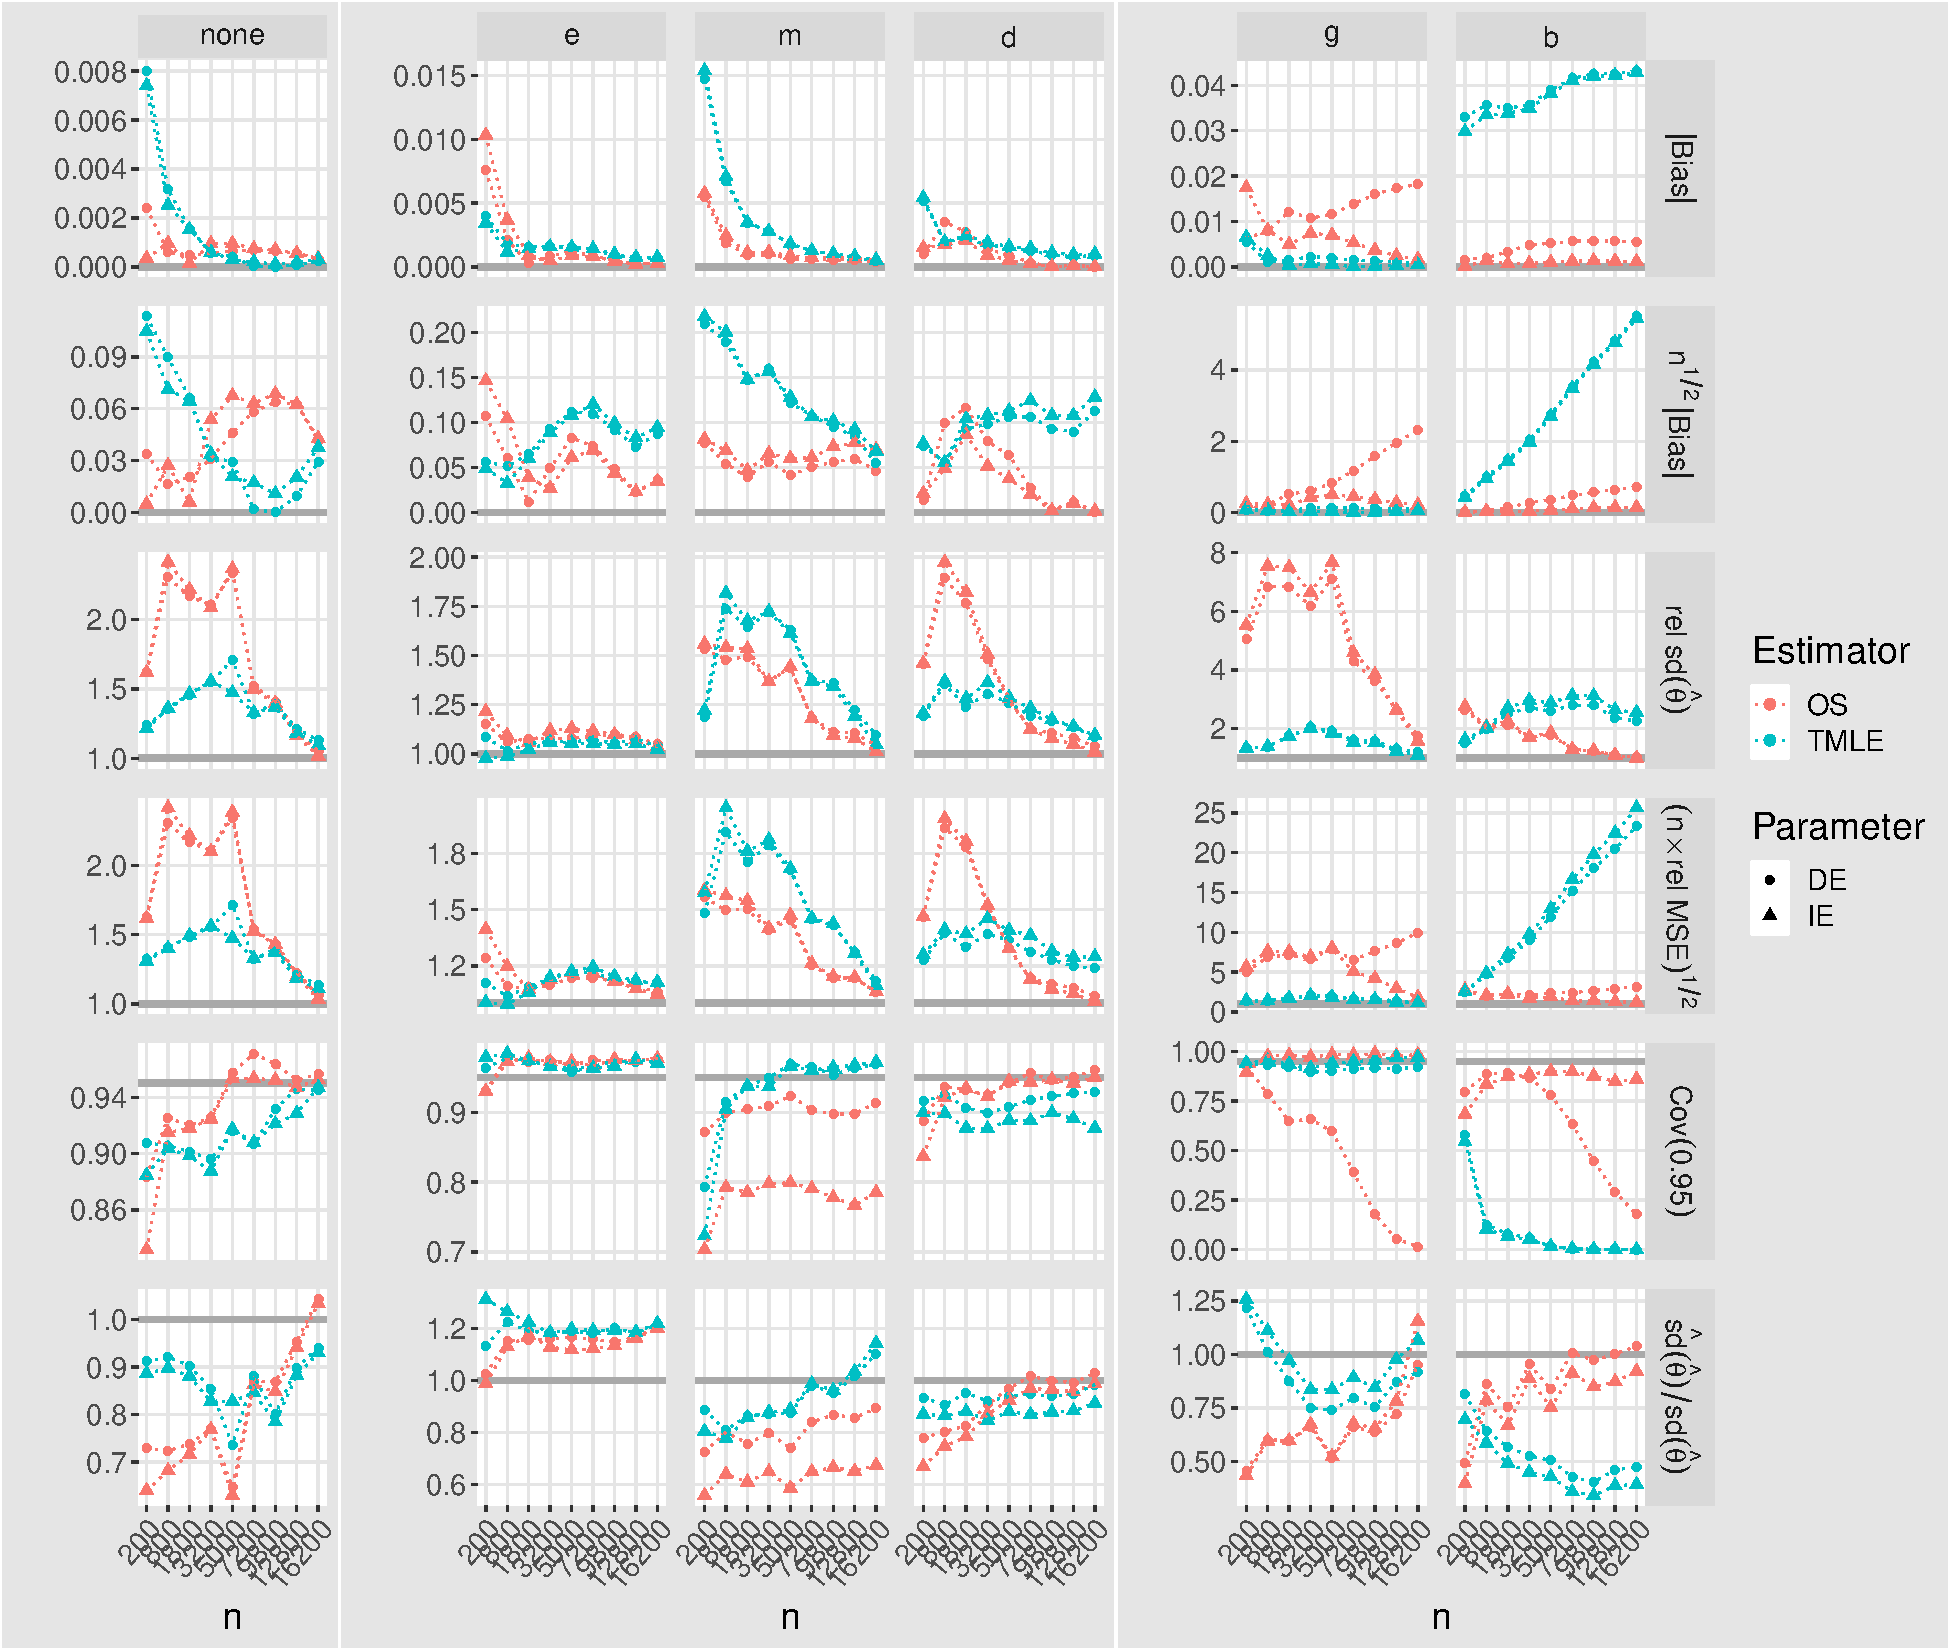
\includegraphics[scale = 0.45]{plot}
  \caption{Comparison of efficient estimators across different nuisance
    parameter configurations.}\label{fig:simula}
\end{figure}
Importantly, the TML estimator appears to generally outperform the one-step
estimator throughout several scenarios. This comes in several forms, including
lower bias, relative standard deviation, or relative mean squared error under
misspecification of $\{\e, \m, \d\}$ or under no misspecification; however,
under inconsistent estimation of $\{\g, \b\}$, the irregularity of the
estimators complicates this comparison. Interestingly, under misspecification of
$\g$, the TML estimators of the direct and indirect effects appear unbiased and
efficient, a result unpredictable from theory given the irregularity of the
estimators under this configuration. Altogether, results of our numerical
experiments indicate that our proposed estimators exhibit properties that align
with the theoretical results of Lemmas~\ref{lemma:dr1} and~\ref{lemma:dr2}.
%while, under similar misspecification of $\b$, the TML estimators exhibit
%diverging bias, an inability to achieve the efficiency bound, and quickly
%diminishing coverage of 95\% confidence intervals. In these latter two cases,
%the irregularity of both the one-step and TML estimators

%%%%%%%%%%%%%%%%%%%%%%%%%%%%%%%%%%%%%%%%%%%%%%%%%%%%%%%%%%%%%%%%%%%%%%%%%%%%%%%
\section{Application to the X:BOT Trial}\label{sec:applic}
%%%%%%%%%%%%%%%%%%%%%%%%%%%%%%%%%%%%%%%%%%%%%%%%%%%%%%%%%%%%%%%%%%%%%%%%%%%%%%%

We now consider the application of our proposed stochastic interventional direct
and indirect effects to decompose the causal effect of a strategy where
buprenorphine dose is successively increased early in treatment (regardless of
opioid use) on relapse among those with opioid use disorder (OUD). Data for our
illustrative analysis come from the X:BOT trial, a 24-week, multi-site
randomized controlled trial designed to examine the comparative effectiveness of
extended-release naltrexone (XR-NTX) and sublingual buprenorphine-naloxone
(BUP-NX) on relapse~\citep{lee2018comparative, lee2016nida, nunes2016ethical}.
The X:BOT trial enrolled 570 participants, all of whom were 18 years or older,
had OUD~\citep[as per the Diagnostic and Statistical Manual of Mental
Disorders-5;][]{apa2013dsm5}, and had used non-prescribed opioids in the 30 days
preceding enrollment. Participants were randomized to receive either XR-NTX or
BUP-NX using a stratified permuted block design; 287 of the 570 were randomized
to receive BUP-NX. Prior analytic efforts have established a protective effect
of BUP-NX administration (versus placebo) on OUD
relapse~\citep{mattick2014buprenorphine}. For each participant assigned to
receive BUP-NX, the prescribed dose was based on both clinical
indication~\citep{lee2018comparative} and clinician judgment. Some clinicians
tended to hold dose constant over time (i.e., a static regimen), while others
increased dose --- either based on clinical assessment or on the hypothesis that
higher doses would result in better outcomes~\citep{nutt2015considerations,
greenwald2003effects, comer2005buprenorphine, heikman2017polydrug}. In this
analysis, we estimated hypothetical stochastic interventional (in)direct effects
to assess the mechanism by which universally ramping up BUP-NX dose early in
treatment (defined as three or more dose increases in the first four weeks of
treatment) could mitigate the risk of OUD relapse.

Baseline covariates ($W$) available in the data included site; gender; age;
race/ethnicity; homeless status; educational attainment; employment status;
marital status; current intravenous drug use; alcohol use disorder; cocaine use
disorder; age at start of heroin use; severity of current opioid use; indicator
of prior OUD treatment; past withdrawal discomfort level; histories of
amphetamine use, sedative use, and cannabis use; weekly cost of primary drug;
whether or not living with an individual currently using drugs or with alcohol
use disorder; histories of psychiatric illnesses; randomization timing; baseline
pain level; baseline depression symptoms. The exposure ($A$) was taken to be
successive increases in dose of BUP-NX versus static dose, measured during the
first four weeks of treatment. Mediating factors ($Z$) included depression and
pain, measured from week 6 until relapse or week 24 (end of follow-up).
Abstinence from illicit opioid use early in the treatment schedule, measured
between weeks 4 and 6, acted as an intermediate confounder affected by exposure
($L$). OUD relapse status at the X:BOT trial's end of follow-up was the outcome
of interest ($Y$). To examine the effect of exposure to successive increases in
BUP-NX dose, we consider an incremental propensity score intervention, which,
for binary $A$, replaces the propensity score $g(1 \mid w)$ with a shifted
variant constructed from multiplying the odds of treatment by a user-specified
parameter $\delta$~\citep{kennedy2019nonparametric}, which we vary along a grid
$\log(\delta) \in \{-10.0, -9.5, \ldots, 9.5, 10.0\}$ of the exposure odds
observed in the X:BOT trial.
%By considering a grid in $\delta$ of plausible incremental propensity score
%interventions, our (in)direct effect estimates are poised to reveal both
%a mechanistic pathway through which adaptive BUP-NX dose can affect OUD
%relapse as well as the interplay of dose strategies (indirectly) with
%pertinent neuropsychiatric sequela.
Across all such estimates in the odds $\delta$ of exposure, the stochastic
interventional (in)direct effects that we estimated may be interpreted
in terms of the overall effect of increasingly encouraging ramping up BUP-NX
dose early in treatment on the counterfactual risk of OUD relapse; thus, the
results of our analysis may be informative of the mechanisms by which increasing
BUP-NX dose can alter the risk of OUD relapse. Figure~\ref{fig:xbot_ipsi}
presents the direct and indirect effect estimates across the grid in $\delta$.
\begin{figure}[H]
  \centering
  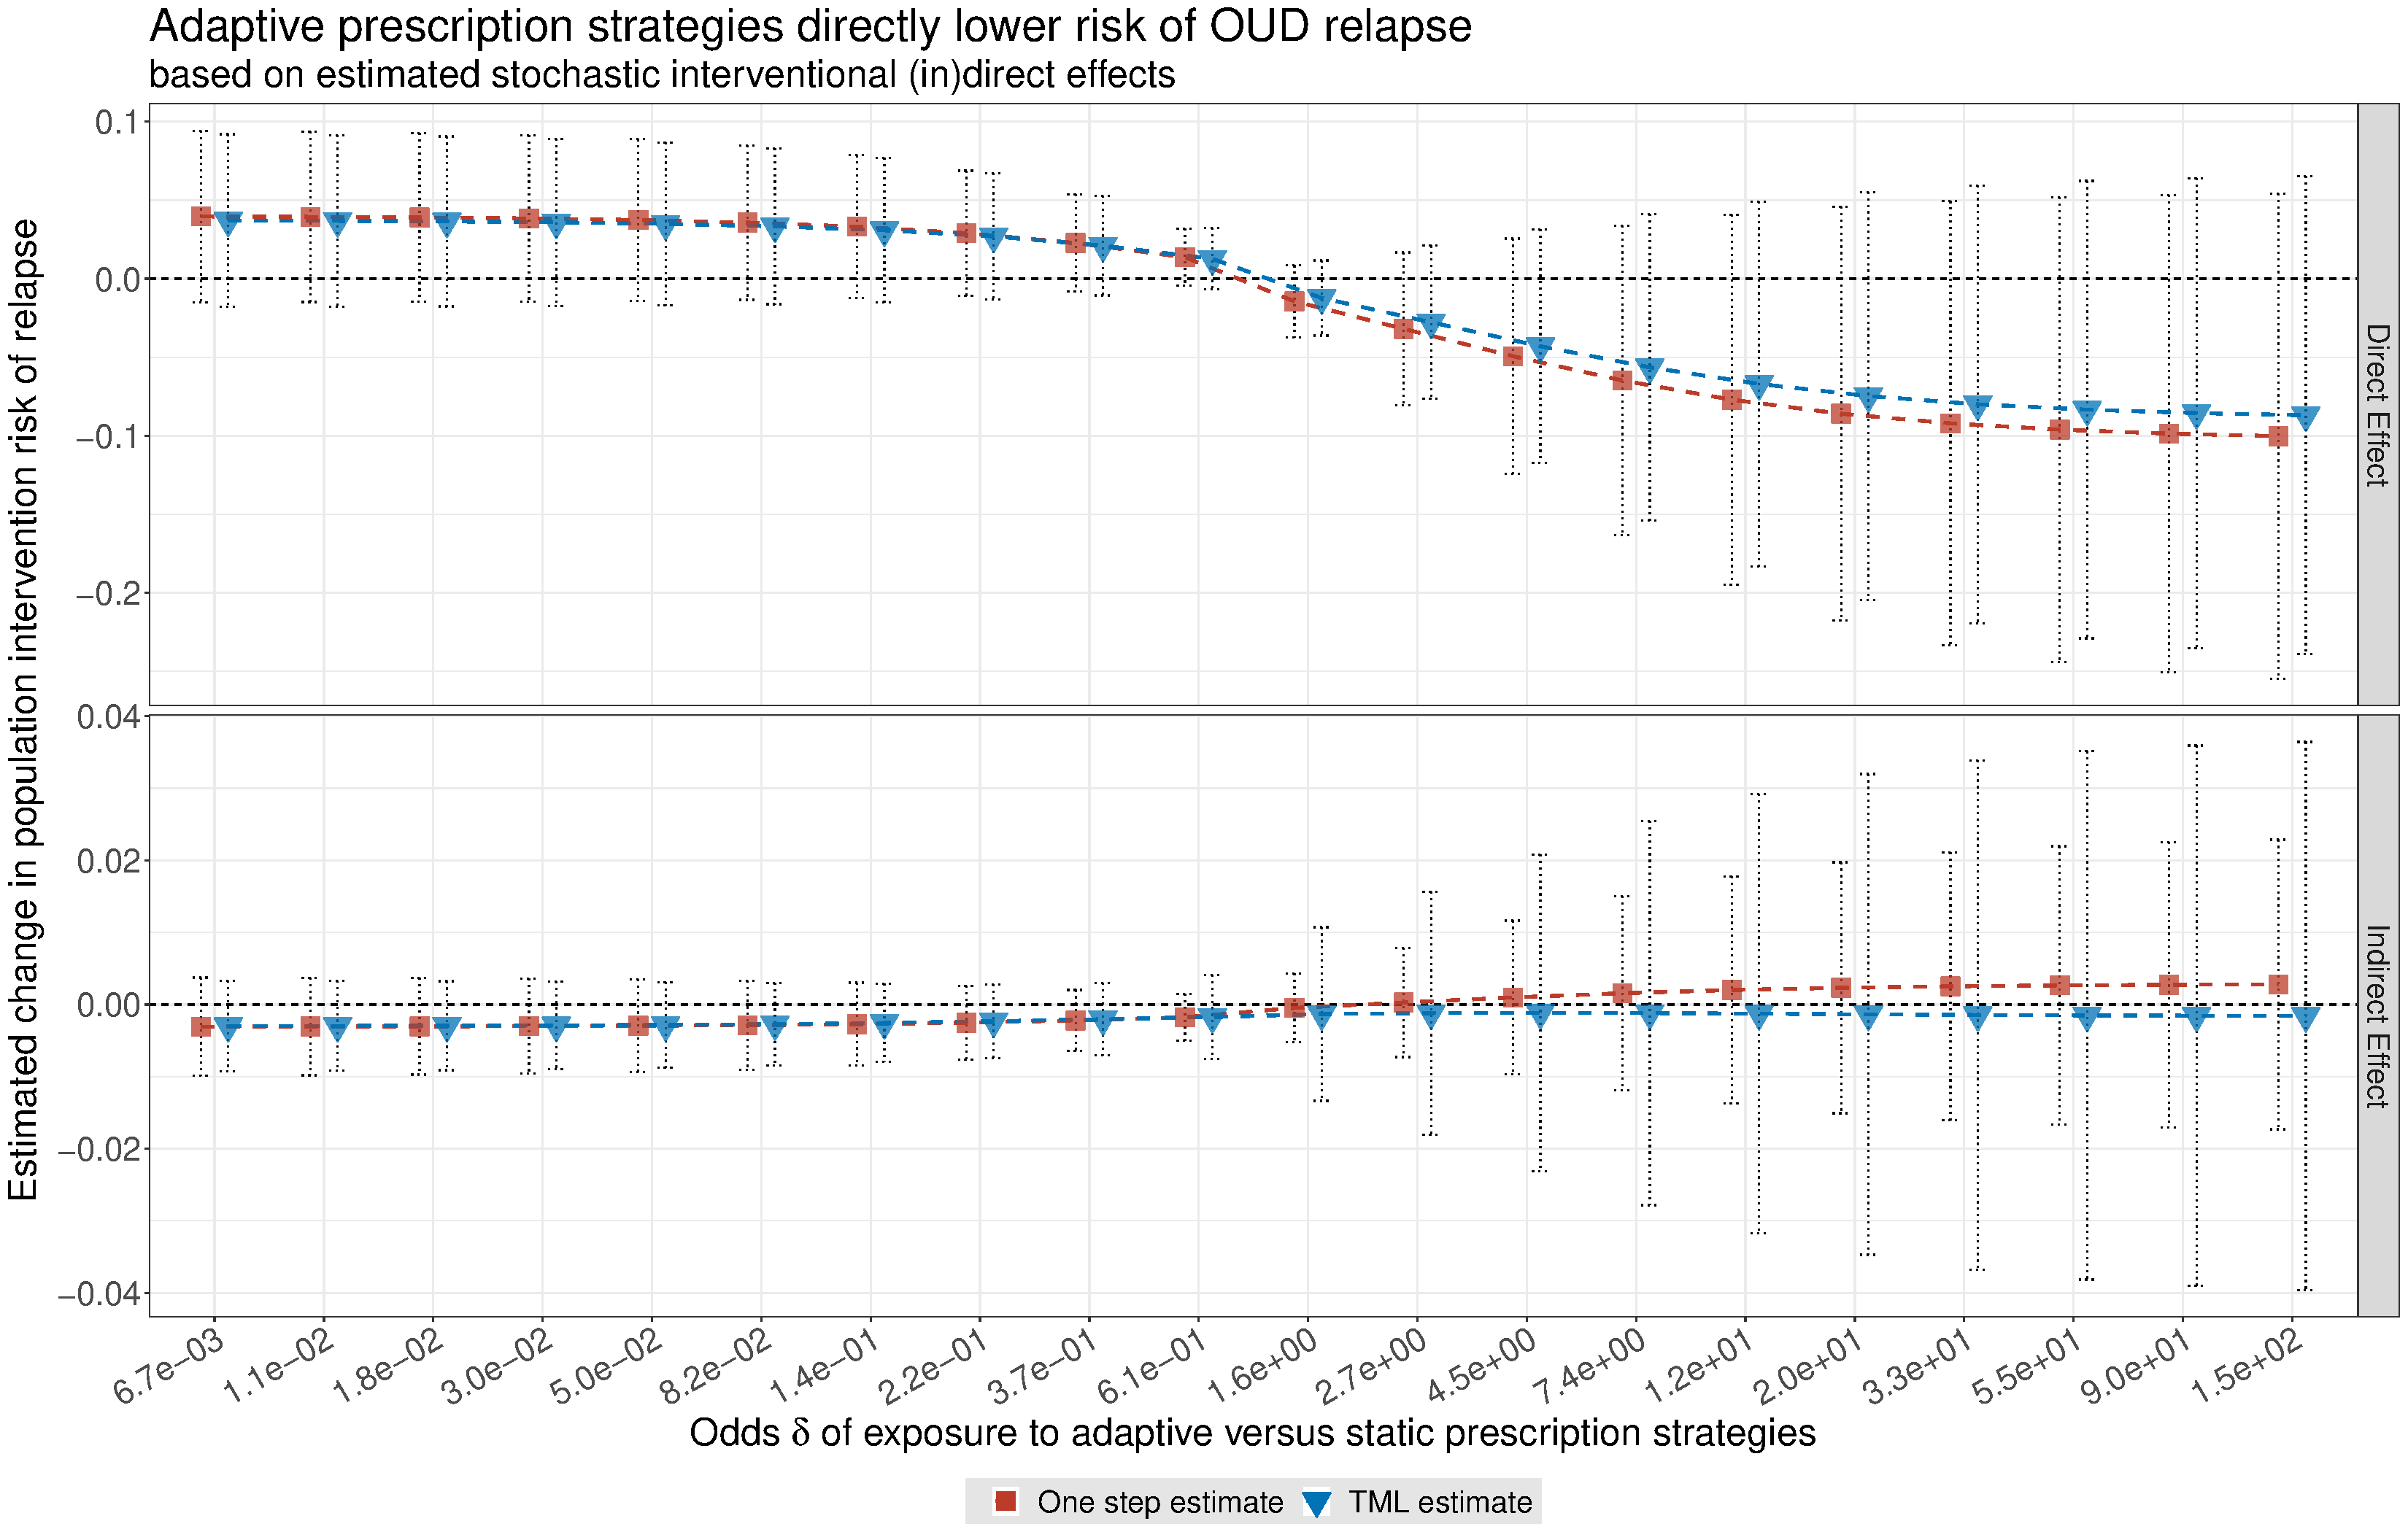
\includegraphics[scale=0.28]{manuscript_xbot}
  \caption{Stochastic interventional direct (upper panel) and indirect (lower
  panel) effect estimates of a hypothetical intervention increasing odds of
  exposure to a BUP-NX dose schedule in which dose is successively increased
  early in OUD relapse treatment across a grid of shifts $\delta$ in the odds.}
  \label{fig:xbot_ipsi}
\end{figure}
We applied both of our cross-fitted, efficient one-step and TML estimators to
examine the stochastic interventional direct and indirect effects of increasing
the odds of ramping up BUP-NX dose. Both estimation strategies produced results
that were generally in very close agreement as to the magnitude of the direct
and indirect effects. For each point estimate, standard error estimates and 95\%
Wald-style confidence intervals were constructed based on the conclusions of
Theorem~\ref{theo:astmle}. In order to ensure the flexibility of our estimators,
each component of the vector of nuisance parameters $\eta = (\e, \m, \d, \g,
\b)$ was estimated via ensemble machine learning, using the Super Learner
algorithm~\citep{vdl2007super, coyle2020sl3}. The library of machine learning
algorithms from which the Super Learner ensemble was constructed included
intercept-only logistic regression, logistic regression with Bayesian priors on
parameters, multivariate adaptive regression
splines~\citep{friedman1991multivariate}, generalized additive
models~\citep{hastie1990generalized}, random forests~\citep{breiman2001random},
gradient boosted machines~\citep{friedman2001greedy}, and the highly adaptive
lasso~\citep{benkeser2016highly, coyle2020hal9001, hejazi2020hal9001}.

From examination of the point estimates and confidence intervals of the direct
and indirect effects in Figure~\ref{fig:xbot_ipsi}, two conclusions may be
drawn. Firstly, there appears to be little to no indirect effect of successively
increasing BUP-NX dose on risk of OUD relapse, revealing that any effect of
BUP-NX dose does not appear to operate through mediating factors such as
depression or pain. Secondly, the direct effect of successively increasing
BUP-NX dose varies considerably across changes in the odds of the introduction
of such a dose schedule. Importantly, it appears that decreasing the odds of
increasing  dose could lead to as much as a 5\% increase in the OUD relapse
risk, with a plateau emerging at odds lower than $\approx$0.1\%, suggesting that
static dose can lead to increased relapse risk relative to successive dose
increases. Continuing this pattern, OUD relapse risk appears to decrease by
$\approx$10\% with increasing odds of successively increasing BUP-NX dose, with
the risk plateauing at odds higher than 33\%. This decrease in the
counterfactual risk of OUD relapse suggests a protective effect of BUP-NX dose
schedules where dose is successively increased early in treatment relative to
static dose.

The conclusions that may be drawn from our re-analysis using the stochastic
interventional direct and indirect effects complement those previously reported
in the investigations of~\citet{lee2018comparative}, who evaluated the total
effect of BUP-NX (versus XR-NTX) treatment on OUD relapse,
and~\citet{rudolph2020explaining}, who used the interventional mediation
analysis approach of~\citet{diaz2020nonparametric} (limited to static
interventions on $A$) to examine differences in relapse risk between homeless
and non-homeless participants. Importantly, our substantive conclusion --- that
dose increases directly lower the risk of relapse --- agree generally with those
of~\citet{rudolph2020association}, who found that dose increases directly
lowered risk of OUD relapse when such dose increases followed opioid use.
Notably, our proposed (in)direct effects and estimation approach differ from
previous efforts in three important ways: (i) our causal effect definitions
remain unaltered in the presence intermediate confounders affected by exposure
and may be re-evaluated in randomized trials, (ii) the flexible estimators we
introduce eschew restrictive modeling assumptions by incorporating
state-of-the-art machine learning in the estimation of nuisance parameters, and
(iii) our strategy provides an analog to a dose-response analysis by allowing
for the risk of OUD relapse to be traced out across changes in the odds of
exposure to a schedule in which BUP-NX dose is increased repeatedly early in
treatment.

%%%%%%%%%%%%%%%%%%%%%%%%%%%%%%%%%%%%%%%%%%%%%%%%%%%%%%%%%%%%%%%%%%%%%%%%%%%%%%%
\section{Discussion}\label{sec:discuss}
%%%%%%%%%%%%%%%%%%%%%%%%%%%%%%%%%%%%%%%%%%%%%%%%%%%%%%%%%%%%%%%%%%%%%%%%%%%%%%%

% Structure adapted from
% https://www.tandfonline.com/doi/pdf/10.1080/01621459.2017.1319839

We have proposed a class of novel direct and indirect effects for causal
mediation analysis, as well as two efficient estimators of these effects in the
nonparametric statistical model. Importantly, our proposed estimation framework
allows for data adaptive estimation of nuisance parameters, while still
preserving the benefits associated with similar classical techniques --- that
is, our estimators are regular and asymptotically linear, provide unbiased point
estimates, are multiply robust, allow the construction of asymptotically valid
confidence intervals, and are capable of attaining the nonparametric efficiency
bound. Our (in)direct effects have interpretations that echo those of the
classical natural (in)direct effects; however, our effects remain well-defined
even in the presence of intermediate confounders affected by exposure. Further,
any scientific conclusions drawn based upon our proposed (in)direct effects may
be readily interrogated in trials that randomize both the exposure and
mediators. Such flexible effect definitions and estimators seem necessary both
to cope with the design complexity exhibited by modern epidemiological and
biomedical studies and to take appropriate advantage of the ever-growing number
of data adaptive regression techniques.

The challenge of leveraging data adaptive regression methodology to construct
robust estimators that accommodate valid statistical inference is not a new one.
It has been considered in great detail as early as the work
of~\citet{pfanzagl1985contributions} as well in numerous recent advances, most
notably by~\citet{vdl2011targeted, vdl2018targeted}
and~\citet{chernozhukov2018double}; related work by these authors presents
a wealth of extensions and applications. In the present work, we derive multiply
robust, efficient estimators based on both the one-step and targeted minimum
loss estimation frameworks. Following~\citet{klaassen1987consistent}
and~\citet{zheng2011cross}, our estimators leverage cross-validation to avoid
imposing possibly restrictive assumptions on nuisance function estimators. We
demonstrated the properties of our estimators in simulation experiments that
illustrated their ability to yield unbiased point estimates, attain the
nonparametric efficiency bound, and build confidence intervals covering at the
nominal rate across several nuisance parameter configurations --- all within a
problem context in which classical mediation effects are ill-defined. We
demonstrated the application of our novel (in)direct effects in dissecting the
mechanism by which increasing odds of adopting a dose schedule of universal
successive increases in buprenorphine dose early in treatment affects OUD
relapse~\citep{lee2018comparative, rudolph2020explaining}.

Several significant extensions and refinements are left for future
consideration. Firstly, our proposed estimation strategy for the direct and
indirect effects leverages re-parameterizations of factors of the likelihood in
order to simplify the estimation of nuisance parameters. This approach works
particularly well when either mediators or intermediate confounders are of low
dimension; however, improving this approach to accommodate moderate
dimensionality of both mediators and intermediate confounders would surely widen
the range of scenarios to which the methodology may be applied. Secondly, when
defining effects based upon stochastic interventions indexed by the
user-specified parameter $\delta$, an important consideration is choosing
\textit{a priori} a particular value of $\delta$. One solution is to evaluate
a set of causal effects indexed by a grid in $\delta$. In such cases, aggregate
effects (across $\delta$) may be summarized via working marginal structural
models~\citep[e.g.,][]{hejazi2020efficient} or the construction of uniform tests
of the null hypothesis of no direct effect~\citep[e.g.,][]{diaz2020causal}.
Developments of these distinct summarization strategies would enrich the range
of scientific problems on which these robust and flexible (in)direct effects may
be brought to bear.

%%%%%%%%%%%%%%%%%%%%%%%%%%%%%%%%%%%%%%%%%%%%%%%%%%%%%%%%%%%%%%%%%%%%%%%%%%%%%%%
\section{Supplementary Materials}\label{sm}
%%%%%%%%%%%%%%%%%%%%%%%%%%%%%%%%%%%%%%%%%%%%%%%%%%%%%%%%%%%%%%%%%%%%%%%%%%%%%%%

\subsection{Theorem \ref{theo:iden}}
\begin{proof}
  % The first part of the Theorem is proved in \cite{Diaz12}. The second part
  % is proved as follows.
  First, we have
  \begin{align}
    \E&\{Y_{A_\delta, G_\delta}\} \notag\\&= \int \E\left\{Y_{a,z}\mid
                                            A_\delta=a,G_\delta = z,
                                            W=w\right\}\g_\delta(a\mid
                                            w)\P(G_\delta=z\mid
                                            A_\delta=a,W=w)\p(w)\dd\nu(a,z,w)\notag\\
      &= \int \E\left\{Y_{a,z}\mid W=w\right\}\g_\delta(a\mid
        w)\P(Z(a)=z\mid
        A_\delta=a,W=w)\p(w)\dd\nu(a,z,w)\label{eq:t1e1}\\
      &= \int \E\left\{Y_{a,z}\mid A=a,W=w\right\}\g_\delta(a\mid
        w)\P(Z(a)=z\mid W=w)\p(w)\dd\nu(a,z,w)\label{eq:t1e2}\\
      &= \int \E\left\{Y_{a,z}\mid A=a,W=w\right\}\g_\delta(a\mid
        w)\P(Z(a)=z\mid A=a,W=w)\p(w)\dd\nu(a,z,w)\label{eq:t1e3}\\
      &= \int \E\left\{Y_{a,z}\mid A=a,W=w,L=l\right\}\b(l\mid a,w)\g_\delta(a\mid
        w)\p(z\mid a,w)\p(w)\dd\nu(a,z,l,w)\notag\\
      &= \int \m(a,z,l,w)\b(l\mid a,w)\g_\delta(a\mid
        w)\p(z\mid a,w)\p(w)\dd\nu(a,z,l,w)\label{eq:t1e4},
  \end{align}
  where (\ref{eq:t1e1}) follows by definition of $(A_\delta,G_\delta)$,
  (\ref{eq:t1e2}) follows by~\ref{ass:ncay} and definition of
  $A_\delta$, (\ref{eq:t1e3}) follows by~\ref{ass:ncaz}, and
  (\ref{eq:t1e4}) follows by~\ref{ass:nczy}. Similar arguments yield
  \[\E\{Y_{A, G}\}=\int \m(a,z,l,w)\b(l\mid a,w)\g(z\mid
    w)\p(z\mid a,w)\p(w)\dd\nu(a,z,l,w).\]
  We also have
  \begin{align*}
    \E&\{Y_{A_\delta, G}\} \notag\\&= \int \E\left\{Y_{a,z}\mid
                                     A_\delta=a,G = z,
                                     W=w\right\}\g_\delta(a\mid
                                     w)\P(G=z\mid
                                     A_\delta=a,W=w)\p(w)\dd\nu(a,z,w)\notag\\
      &= \int \E\left\{Y_{a,z}\mid W=w\right\}\g_\delta(a\mid
        w)\P(G=z\mid W=w)\p(w)\dd\nu(a,z,w)\\
      &= \int \E\left\{Y_{a,z}\mid A=a,W=w\right\}\g_\delta(a\mid
        w)\p(z\mid w)\p(w)\dd\nu(a,z,w)\\
      &= \int \E\left\{Y_{a,z}\mid A=a,W=w\right\}\g_\delta(a\mid
        w)\p(z\mid w)\p(w)\dd\nu(a,z,w)\\
      &= \int \E\left\{Y_{a,z}\mid A=a,W=w,L=l\right\}\b(l\mid a,w)\g_\delta(a\mid
        w)\p(z\mid w)\p(w)\dd\nu(a,z,l,w)\notag\\
      &= \int \m(a,z,l,w)\b(l\mid a,w)\g_\delta(a\mid
        w)\p(z\mid w)\p(w)\dd\nu(a,z,l,w).
  \end{align*}
  Subtracting gives the expressions for the PIIE and PIDE in the
  theorem.
\end{proof}

\subsection{Efficient influence functions (Theorem~\ref{theo:eif})}
\begin{proof}
  In this proof we will use $\Theta_j(\P):j=1,2$ to denote a parameter
  as a functional that maps the distribution $\P$ in the model to a
  real number. We will assume that the measure $\nu$ is discrete so
  that integrals can be written as sums, and will omit the dependence
  on $\delta$. It can be checked algebraically that the resulting
  influence function will also correspond to the influence function of
  a general measure $\nu$. The true parameter value for $\theta_1$ is
  thus given by
  \[\theta_1=\Theta_1(\P) = \sum_{y,a,z,m,w} y\,\p(y\mid a, z, l,
    w)\p(l\mid a,w)\p(z\mid a,w)\g_\delta(a\mid w)\p(w).\] The
  non-parametric MLE of $\theta_1$ in the model of $\g_\delta$ known
  is given by
  \begin{equation}
    \Theta(\Pn)=\sum_{y,a,z,m,w}y\frac{\Pn f_{y,a,z,l,w}}{\Pn
      f_{a,z,l,w}}\frac{\Pn f_{l,a,w}}{\Pn f_{a,w}}\frac{\Pn
      f_{z,a,w}}{\Pn f_{a,w}}\g_{\delta}(a\mid w)\Pn f_w\label{nonpest},
  \end{equation}
  where we remind the reader of the notation $\P f =\int f \dd\P$. Here
  $f_{y,a,z,l,w}=\one(Y=y,A=a,Z=z,M=m,W=w)$, and $\one(\cdot)$ denotes
  the indicator function. The other functions $f$ are defined
  analogously.

  We will use the fact that the efficient influence function in a
  non-parametric model corresponds with the influence curve of the
  NPMLE. This is true because the influence curve of any regular
  estimator is also a gradient, and a non-parametric model has only
  one gradient. The Delta method \cite[see, e.g., Appendix 18
  of][]{vdl2011targeted} shows that if $\hat \Theta_1(\Pn)$ is a
  substitution estimator such that $\theta_1=\hat \Theta_1(\P)$, and
  $\hat \Theta_1(\Pn)$ can be written as
  $\hat \Theta^*_1(\Pn f:f\in\mathcal{F})$ for some class of functions
  $\mathcal{F}$ and some mapping $\Theta^*_1$, the influence function of
  $\hat \Theta_1(\Pn)$ is equal to
  \[\dr_\P(O)=\sum_{f\in\mathcal{F}}\frac{\dd\hat \Theta^*_1(\P)}
  {\dd\P f}\{f(O)-\P f\}.\]

  Applying this result to (\ref{nonpest}) with
  $\mathcal{F}=\{f_{y,a,z,l,w},f_{a,z,l,w},f_{z,a,w},f_{a',w},
  f_{l,a,w},f_{a,w},f_w:y,a,z,l,w\}$ and rearranging terms gives the result of
  the theorem. The algebraic derivations involved here are lengthy and not
  particularly illuminating, and are therefore omitted from the proof. Similar
  analyses may be performed for the model where only $\g_\delta$ is unknown, as
  well as $\theta_2$.
\end{proof}

\subsection{Targeted minimum loss estimation algorithm}

To simplify notation, in the remaining of this section we will denote
$\tilde \eta_{j(i)}(O_i)$ with $\tilde \eta(O_i)$. If $L$ is binary,
the efficient influence functions in Theorem~\ref{theo:eif} may be
simplified using the following identity:
\[ \vv(l,a,w) - \bar\vv(a,w) = \{\vv(1,a,w) -\vv(0,a,w)\}
\{l-\b(1\mid a, w)\},\] which also holds for $\vv$ replaced by $\s$ and
$\bar\vv$ by $\bar\s$.

\begin{enumerate}[label=Step \arabic*., align=left, leftmargin=*]
\item Initialize $\tilde\eta =\hat\eta$. Compute $\tilde\vv$,
  $\tilde\s$, and $\tilde\q^j$ by plugging in $\tilde \m$,
  $\tilde \g$, $\tilde \e$, $\tilde \d$ into equations
  (\ref{eq:nuis}), (\ref{eq:altnuis}) and (\ref{eq:defqs}) if
  $Z$ is multivariate, and fitting data-adaptive regression algorithms as
  appropriate.

\item \label{step:computeH} For each subject, compute the auxiliary covariates
  \begin{align*}
    H_{\mbox{\scriptsize D}, i} &= \frac{{\tilde\b}(L_i\mid A_i,
                                  W_i)}{{\tilde\d}(L_i \mid Z_i, A_i,
                                  W_i)}\left\{1-\frac{{\tilde\g}_\delta(A_i\mid
                                  W_i)}{{\tilde\e}(A_i\mid Z_i,W_i)}\right\}\\
    H_{\mbox{\scriptsize I}, i} &= \frac{{\tilde\b}(L_i\mid A_i,
                                  W_i)}{{\tilde\d}(L_i \mid Z_i, A_i,
                                  W_i)}\left\{\frac{{\tilde\g}_\delta(A_i\mid
                                  W_i)}{{\tilde\e}(A_i\mid
                                  Z_i,W_i)}-\frac{\tilde{\g}_\delta(A_i
                                  \mid W_i)}{{\tilde\g}(A_i\mid
                                  W_i)}\right\}\\
    K_{\mbox{\scriptsize D}, i} & = {\tilde\vv}(1,A_i,W_i)
                                  - {\tilde\vv}(0,A_i,W_i) - \frac{{\tilde\g}_\delta(A_i
                                  \mid W_i)}{{\tilde\g}(A_i\mid W_i)} \{{\tilde\s}(1,A_i,W_i) -
                                  {\tilde\s}(0,A_i,W_i)\}\\
    K_{\mbox{\scriptsize I}, i} & = \frac{{\tilde\g}_\delta(A_i
                                  \mid W_i)}{{\tilde\g}(A_i\mid W_i)}
                                  \{{\tilde\s}(1,A_i,W_i) -
                                  {\tilde\s}(0,A_i,W_i) - {\tilde\vv}(1,A_i,W_i)
                                  + {\tilde\vv}(0,A_i,W_i)\}\\
    M_{\mbox{\scriptsize D}, i} & = -\frac{\tilde\g_\delta(1\mid w)(1 -
                                  \tilde\g_\delta(1\mid w))}{\tilde\g(1\mid w)(1 -
                                  \tilde\g(1\mid w))}{\tilde\q}^2(w)\\
    M_{\mbox{\scriptsize I}, i} & = \frac{\tilde\g_\delta(1\mid w)(1 -
                                  \tilde\g_\delta(1\mid w))}{\tilde\g(1\mid w)(1 -
                                  \tilde\g(1\mid w))}\{{\tilde\q}^2(w)-{\tilde\q}^1(w)\}
  \end{align*}
\item \label{step:fit} Fit the logistic tilting models
  \begin{align*}
    \logit \m_\beta(A_i,Z_i,L_i,W_i) &= \logit \tilde
                                       \m(A_i,Z_i,L_i,W_i) + \beta_I H_{\mbox{\scriptsize I}, i} +
                                       \beta_D H_{\mbox{\scriptsize D}, i}\\
    \logit \b_\alpha(1\mid A_i,W_i) &= \logit \tilde
                                      \b(1\mid A_i,W_i) + \alpha_I K_{\mbox{\scriptsize I}, i} +
                                      \alpha_D K_{\mbox{\scriptsize
                                      D}, i}\\
    \logit \g_\gamma(1\mid W_i) &= \logit \tilde
                                  \g(1\mid W_i) + \gamma_I M_{\mbox{\scriptsize I}, i} +
                                  \gamma_D M_{\mbox{\scriptsize D}, i}
  \end{align*}
  where
  $\logit(p) = \log\{p(1-p)^{-1}\}$. Here, $\logit \tilde\m(a,z,l,w)$
  is an offset variable (i.e., a variable with known parameter value
  equal to one). The parameter $\beta=(\beta_I, \beta_D)$ may be
  estimated by running standard logistic regression of $Y_i$ on
  $(H_{\mbox{\scriptsize D}, i}, H_{\mbox{\scriptsize I}, i})$ with no
  intercept and an offset term equal to
  $\logit \tilde\m(A_i,Z_i,L_i,W_i)$. Let $\hat\beta$ denote the
  estimate, and let $\tilde \m=\m_{\hat\beta}$ denote the updated
  estimates. Perform analogous computations for $\b$ and $\g$.
\item \label{step:computeu} Compute $\tilde\uu$ according to equation
  (\ref{eq:nuis}) by plugging in $\tilde\m$ and $\tilde\b$. Compute
  the covariate
  \[J_i = \frac{{\tilde\g}_\delta(A_i
      \mid W_i)}{{\tilde\g}(A_i\mid W_i)},\]
  and fit the model
  \[\logit \bar\uu_\kappa(A_i,W_i) = \logit \tilde{\bar\uu}(A_i,W_i) +
    \kappa_D + \kappa_I J_{ i}\] by running a logistic regression of
  $\tilde\uu(Z_i,A_i,W_i)$ on $J_i$ with an intercept and offset
  $\logit \tilde{\bar\uu}(A_i,W_i)$. Let $\hat\kappa$ denote the MLE,
  and update $\tilde{\bar\uu} = \bar\uu_{\hat \kappa}$.
\item The TMLE of the direct and indirect effects are defined as:
  \begin{equation*}
    \begin{split}
      \psidtmle &= \frac{1}{n} \int\sum_{i = 1}^n
      \left\{\tilde{\bar\uu}(a,W_i)\tilde\g(a\mid W_i) -
        \tilde\uu(Z_i,a,W_i)\tilde\g_\delta(a\mid W_i)\right\}\dd\kappa(a)\\
      \psiitmle &= \frac{1}{n} \int\sum_{i = 1}^n
      \left\{\tilde\uu(Z_i,a,W_i) -
        \tilde{\bar\uu}(a,W_i)\right\}\tilde\g_\delta(a\mid
      W_i)\dd\kappa(a)
    \end{split}
  \end{equation*}
\end{enumerate}

\subsection{Proof of Theorem \ref{theo:asos}}
\begin{proof}
  Let $\Pnj$ denote
  the empirical distribution of the prediction set ${\cal V}_j$, and let
  $\Gnj$ denote the associated empirical process
  $\sqrt{n/J}(\Pnj-\P)$. For simplicity we denote a general parameter
  $\psi$ with influence function $D_\eta$, the proof applies equally
  to the direct and indirect effect parameters. Note that
  \[\psios = \frac{1}{J}\sum_{j=1}^J\Pnj D_{\hat
      \eta_j,\delta},\,\,\,\psi_\delta=\P D_{\eta}.\]Thus,
  \[  \sqrt{n}\{\psios - \psi_\delta\}=\Gn \{D_{\eta,\delta}
    - \psi_\delta\} + R_{n,1}(\delta) + R_{n,2}(\delta),\]
  where
  \[  R_{n,1}(\delta)  =\frac{1}{\sqrt{J}}\sum_{j=1}^J\Gnj(D_{\hat
      \eta_j,\delta} - D_{\eta,\delta}),\,\,\,
    R_{n,2}(\delta)  = \frac{\sqrt{n}}{J}\sum_{j=1}^J\P\{D_{\hat
      \eta_j,\delta}-\psi_\delta\}.
  \]
  It remains to show that $R_{n,1}(\delta)$ and $R_{n,2}(\delta)$ are
  $o_P(1)$. Lemmas~\ref{lemma:dr1} and~\ref{lemma:dr2} together
  with the Cauchy-Schwartz inequality and assumption \ref{ass:sec1}
  of the theorem shows that $||R_{n,2}||_{\Delta}=o_P(1)$. For
  $||R_{n,1}||_{\Delta}$ we use empirical process theory to argue conditional
  on the training sample ${\cal T}_j$. In particular, Lemma 19.33
  of~\cite{vdvaart2000asymptotic} applied to the class of functions
  ${\cal F} = \{D_{\hat \eta_j,\delta} - D_{\eta,\delta}\}$ (which
  consists of one element) yields
  \[E\left\{\big|\Gnj (D_{\hat \eta_j,\delta} - D_{\eta,\delta})\big|
      \,\bigg|\, {\cal T}_j\right\}\lesssim \frac{2C\log 2}{n^{1/2}} +
    ||D_{\hat \eta_j,\delta} - D_{\eta,\delta}||(\log 2)^{1/2}\] By
  assumption \ref{ass:sec1}, the left hand side is $o_P(1)$. Lemma 6.1
  of~\cite{chernozhukov2018double} may now be used to argue that
  conditional convergence implies unconditional convergence, concluding
  the proof.
\end{proof}

\subsection{Theorem~\ref{theo:astmle}}
\begin{proof}
  Let $\Pnj$ denote the empirical distribution of the prediction set
  ${\cal V}_j$, and let $\Gnj$ denote the associated empirical process
  $\sqrt{n/J}(\Pnj-\P)$. For simplicity we denote a general parameter
  $\psi$ with influence function $D_\eta$, the proof applies equally
  to the direct and indirect effect parameters. By definition, the sum
  of the scores of the submodels
  $\{\m_\beta,\b_\alpha,\g_\gamma,\bar\uu_\kappa:(\beta,\alpha,
  \gamma, \kappa)\}$ at the last iteration of the TMLE procedure is
  equal to
  $n^{-1}\sum_{i=1}^n D_{\tilde \eta}(O_i) = o_P(n^{-1/2})$. Thus, we have
  \[\psitmle = \frac{1}{J}\sum_{j=1}^J\Pnj D_{\tilde \eta_j}+o_P(n^{-1/2}).\]
  Thus,
  \[  \sqrt{n}(\psitmle - \theta)=\Gn (D_{\eta}
    - \theta) + R_{n,1} + R_{n,2} + o_P(n^{-1/2}),\]
  where
  \[  R_{n,1}  =\frac{1}{\sqrt{J}}\sum_{j=1}^J\Gnj(D_{\tilde
      \eta_j} - D_{\eta}),\,\,\,
    R_{n,2}  = \frac{\sqrt{n}}{J}\sum_{j=1}^J\P(D_{\tilde
      \eta_j}-\theta).
  \]
  As in the proof of Theorem~\ref{theo:asos}, Lemmas~\ref{lemma:dr1}
  and~\ref{lemma:dr2} together with the Cauchy-Schwartz inequality and
  the assumptions of the theorem shows that $R_{n,2}=o_P(1)$.

  Since $D_{\tilde \eta_j}$ depends on the full sample through the
  estimates of the parameters $\beta$ of the logistic tilting models,
  the empirical process treatment of $R_{n,1}$ needs to be slightly
  from that in the proof of Theorem~\ref{theo:asos}. To make this
  dependence explicit, we introduce the notation
  $D_{\hat \eta_j,\beta}=D_{\tilde \eta_j}$ and $R_{n,1}(\beta)$. Let
  ${\cal F}_n^j=\{D_{\hat \eta_j,\beta} -
  D_\eta:\beta\in B\}$. Because the function
  $\hat\eta_j$ is fixed given the training data, we can apply Theorem
  2.14.2 of~\cite{vdvaart1996weak} to obtain
  \[E\left\{\sup_{f\in {\cal F}_n^j}|\Gnj f| \,\,\bigg|\,\, {\cal
        T}_j\right\}\lesssim ||F^j_n||\int_0^1\sqrt{1+N_{[\,]}(\epsilon
      ||F_n^j||, {\cal F}_n^j, L_2(\P))}\dd\epsilon, \] where
  $N_{[\,]}(\epsilon ||F_n^j||, {\cal F}_n^j, L_2(\P))$ is the
  bracketing number and we take
  $F_n^j=\sup_{\beta\in B}|D_{\hat \eta_j,\beta} -
  D_\eta|$ as an envelope for the class ${\cal
    F}_n^j$. Theorem 2.7.2 of~\cite{vdvaart1996weak} shows
  \[\log N_{[\,]}(\epsilon ||F_n^j||, {\cal F}_n^j, L_2(\P))\lesssim
    \frac{1}{\epsilon ||F_n^j||}.\]
  This shows
  \begin{align*}||F^j_n||\int_0^1\sqrt{1+N_{[\,]}(\epsilon
    ||F_n^j||, {\cal F}_n^j, L_2(\P))}\dd\epsilon &\lesssim
        \int_0^1\sqrt{||F^j_n||^2+\frac{||F^j_n||}{\epsilon}}\dd\epsilon\\
        &\leq
    ||F^j_n||+||F^j_n||^{1/2}\int_0^1\frac{1}{\epsilon^{1/2}}\dd\epsilon\\
        &\leq ||F^j_n|| + 2 ||F^j_n||^{1/2}.
  \end{align*}
  Since $||F^j_n||=o_P(1)$, this shows
  $\sup_{f\in {\cal F}_n^j}\Gnj f=o_P(1)$ for each $j$, conditional on
  ${\cal T}_j$. Thus $\sup_{\beta\in B} R_{n,1}(\beta)=o_P(1)$.
  Lemmas~\ref{lemma:dr1} and~\ref{lemma:dr2} together with the
  Cauchy-Schwartz inequality and the assumptions of the theorem show
  that $R_{n,2}=o_P(1)$, concluding the proof of the theorem.
\end{proof}

\subsection{Additional results}

\begin{lemma}[Second order terms for modified treatment
  policies]\label{lemma:so1}
  Let $\dd\xi(o)$ denote $\dd\nu(a,l,z)\dd\P(w)$, and let $\r(z\mid,
  a, w)$ denote $\p(z\mid a, w)$, and let $\h(z\mid,
  w)$ denote $\p(z\mid w)$. Let $d(a,w)$ denote a modified treatment
  policy satisfying~\ref{ass:inv}. We have
  \begin{align}
    \P D_{\eta_1,\delta}^1 -\psi_1(\delta) & =
         \int\left(\frac{\g}{\g_1}\frac{\d}{\d_1} -
        1\right)(\m-\m_1)\b_1\r\g_{\delta,1}\dd\xi\label{eq:so1}\\
        &-\int\left(\frac{\g}{\g_1}-1\right)(\bar\uu_1-\bar\uu)
        \g_{\delta,1}\dd\xi\label{eq:so3}\\
         &+\int\left(\frac{\g}{\g_1}-1\right)(\m_1-\m)\b_1\r
         \g_{\delta,1}\dd\xi\label{eq:so4}\\
         &-\int\frac{\g}{\g_1}(\b_1-\b)(\vv_1-\vv)\g_{\delta,1}
         \dd\xi\label{eq:so5}\\
        &-\int(\bar\uu_1-\bar\uu)(\g_{\delta,1}-\g_\delta)
        \dd\xi\label{eq:so2}
  \end{align}
  and
  \begin{align*}
    \P D_{\eta_1,\delta}^2 - \psi_2(\delta)
    & = \int\left(\frac{\e}{\e_1}\frac{\d}{\d_1} -
      1\right)(\m-\m_1)\b_1\h\g_{\delta,1} \dd\xi\\
    &+\int\frac{\g}{\g_1}(\b_1-\b)(\s_1-\s)\g_{\delta,1}\dd\xi\\
    &-\int(\q_1-\q)(\g_{\delta,1}-\g_\delta)\dd\xi.
  \end{align*}
\end{lemma}
\begin{proof} Note that
\begin{equation}
  \begin{split}
    \P S_{\eta_1,\delta}^1 -
    \psi_1(\delta)
    & =
      \int\left(\frac{\g}{\g_1}\frac{\d}{\d_1}
      - 1\right)(\m-\m_1)\b_1\r\g_{\delta,1}\dd\xi
      + \int(\m-\m_1)\b_1\r\g_{\delta,1}\dd\xi                                  \\
    & - \int\bar\uu
      (\g_\delta - \g_{\delta,1})\dd\xi - \int \bar\uu
      \g_{\delta,1}\dd\xi                                                       \\
    & +\int
      \frac{\g}{\g_1}(\b-\b_1)\vv_1\g_{\delta,1}\dd\xi
      + \int
      \frac{\g}{\g_1}(\uu_1\r-\bar\uu_1)\g_{\delta,1}\dd\xi
      +\int\bar\uu_1\g_{\delta,1}\dd\xi                                         \\
    & =(\ref{eq:so1})
      +\int (\bar\uu_1-\bar\uu)\g_{\delta,1}\dd\xi                              \\
    & +\int(\m-\m_1)\b_1\r\g_{\delta,1}\dd\xi +
      \int\frac{\g}{\g_1}(\b-\b_1)\vv_1\g_{\delta,1}\dd\xi                      \\
    & + \int
      \frac{\g}{\g_1}\uu_1\r\g_{\delta,1}\dd\xi
      -\int
      \frac{\g}{\g_1}\bar\uu_1\g_{\delta,1}\dd\xi                               \\
    & - \int\bar\uu
      (\g_\delta - \g_{\delta,1})\dd\xi           \\
    & =(\ref{eq:so1})
      -\int\left(\frac{\g}{\g_1}-1\right)(\bar\uu_1-\bar\uu)\g_{\delta,1}\dd\xi \\
    & +\int \frac{\g}{\g_1}\m_1\b_1\r\g_{\delta,1}\dd\xi - \int
      \frac{\g}{\g_1}\m\b\r\g_{\delta,1}\dd\xi                                  \\
    & +\int(\m-\m_1)\b_1\r\g_{\delta,1}\dd\xi +
      \int\frac{\g}{\g_1}(\b-\b_1)\vv_1\g_{\delta,1}\dd\xi                      \\
    & - \int\bar\uu
      (\g_\delta - \g_{\delta,1})\dd\xi           \\
    & =(\ref{eq:so1})-
      (\ref{eq:so3}) \\
    & +\int(\m-\m_1)\b_1\r\g_{\delta,1}\dd\xi +
      \int\frac{\g}{\g_1}(\b-\b_1)\vv_1\g_{\delta,1}\dd\xi            \\
    & +\int
      \frac{\g}{\g_1}(\m_1\b_1
      +\m\b_1-\m\b_1-
      \m\b)\r\g_{\delta,1}\dd\xi                                      \\
    & - \int\bar\uu
      (\g_\delta - \g_{\delta,1})\dd\xi \\
    & =(\ref{eq:so1}) - (\ref{eq:so3})                                                  \\
    & +
      \int(\m-\m_1)\b_1\r\g_{\delta,1}\dd\xi +
      \int\frac{\g}{\g_1}(\b-\b_1)\vv_1\g_{\delta,1}\dd\xi            \\
    & +\int
      \frac{\g}{\g_1}(\m_1
      -\m)\b_1\r\g_{\delta,1}\dd\xi
      +\int
      \frac{\g}{\g_1}(\b_1-\b)\m\r\g_{\delta,1}\dd\xi                 \\
    & - \int\bar\uu
      (\g_\delta - \g_{\delta,1})\dd\xi \\
    & =(\ref{eq:so1})-(\ref{eq:so3}) +(\ref{eq:so4})-(\ref{eq:so5}) \\
    & - \int\bar\uu(\g_\delta - \g_{\delta,1})\dd\xi.
  \end{split}\label{eq:proof1}
\end{equation}
Using~\ref{ass:inv} we can change variables to obtain
\[\P S_{\eta_1,\delta}^{A,1} =
  \int\bar\uu_1(\g_\delta-\g_{\delta,1})\dd\xi.\] The proof for
$\psi_2$ is analogous. This completes the
proof of the theorem.
\end{proof}

\begin{lemma}[Second order terms for
  exponential tilting.]\label{lemma:so2}
  Define $c(w) = \{\int_a \exp(\delta a)\g(a\mid w)\}^{-1}$, and let
  $c_1(w)$ be defined analogously. Let $b(a) = \exp(\delta a)$. Using
  the same notation as in Lemma~\ref{lemma:dr1}, we have
  \begin{align*}
    \P D_{\eta_1,\delta}^1  -\psi_1(\delta)
    & =
      \int\left(\frac{\g}{\g_1}\frac{\d}{\d_1} -
      1\right)(\m-\m_1)\b_1\r\g_{\delta,1}\dd\xi\\
    &-\int\left(\frac{\g}{\g_1}-1\right)(\bar\uu_1-\bar\uu)\g_{\delta,1}\dd\xi\\
    &+\int\left(\frac{\g}{\g_1}-1\right)(\m_1-\m)\b_1\r\g_{\delta,1}\dd\xi\\
    &-\int\frac{\g}{\g_1}(\b_1-\b)(\vv_1-\vv)\g_{\delta,1}\dd\xi\\
    &+ \int(\bar\uu_1-\bar\uu)(\g_{\delta,1}-\g_\delta)\dd\xi\\
    & -\int\left\{(c_1-c)^2\int b
      \g_1\bar\uu_1\dd\kappa\int b
      \g\dd\kappa\right\}\dd\xi\\
    &+\int \left\{(c_1-c)\int b\bar\uu_1(\g-\g_1)\dd\kappa\right\}\dd\xi,
  \end{align*}
  and
  \begin{align*}
    \P D_{\eta_1,\delta}^2  -\psi_2(\delta)
    & = \int\left(\frac{\e}{\e_1}\frac{\d}{\d_1}  -
      1\right)(\m-\m_1)\b_1\h\g_{\delta,1} \dd\xi\\
    &+\int\frac{\g}{\g_1}(\b_1-\b)(\s_1-\s)\g_{\delta,1}\dd\xi\\
    &-\int(\q_1-\q)(\g_{\delta,1}-\g_\delta)\dd\xi\\
    & -\int\left\{(c_1-c)^2\int b
      \g_1\bar\q_1\dd\kappa\int b
      \g\dd\kappa\right\}\dd\xi\\
    &+\int \left\{(c_1-c)\int b\bar\q_1(\g-\g_1)\dd\kappa\right\}\dd\xi.
  \end{align*}

\end{lemma}

\begin{proof}
  In this proof, (\ref{eq:proof1}) is also valid. We have
  \[\P S_{\eta_1,\delta}^{1,A} - \int\bar\uu(\g_\delta -
    \g_{\delta,1})\dd\xi = \P S_{\eta_1,\delta}^{1,A} - \int\bar\uu_1(\g_\delta -
    \g_{\delta,1})\dd\xi + \int(\bar\uu_1-\bar\uu)(\g_{\delta,1}-\g_\delta)\dd\xi\]
It thus remains to
  prove that
  \begin{align*}
    \P S_{\eta_1,\delta}^{1,A} - \int\bar\uu_1(\g_\delta -
    \g_{\delta,1})\dd\xi = & -\int\left\{(c_1-c)^2\int b
      \g_1\bar\uu_1\dd\kappa\int b
      \g\dd\kappa\right\}\dd\xi\\
    &+\int \left\{(c_1-c)\int b\bar\uu_1(\g-\g_1)\dd\kappa\right\}\dd\xi.
  \end{align*}
  We have
  \begin{align}
    \P S_{\eta_1}^{1,A} -
    & \int\bar\uu_1(\g_{\delta}-\g_{\delta,1})\dd\xi\notag\\
    &=\int\left\{\int\frac{\g_{1,\delta}}{\g_1}\bar\uu_1 \g\dd\kappa
      -\int \frac{\g_{1,\delta}}{\g_1}\g\dd\kappa\int\bar\uu_1 \g_{1,\delta}\dd\kappa + \int(\g_{1,\delta} -
      \g_\delta)\bar\uu_1\dd\kappa\right\}\dd\xi\notag\\
    &=\int\left\{\frac{\g_{1,\delta}}{\g_1}\g\bar\uu_1\dd\kappa - \int \g_\delta\bar\uu_1\dd\kappa + \int
      \g_{1,\delta}\bar\uu_1\dd\kappa\left[1-\int\frac{\g_{1,\delta}}{\g_1}\g\dd\kappa\right]\right\}
      \dd\xi\notag\\
    &=\int\left\{c_1\int
      b\bar\uu_1 \g\dd\kappa
      - c_1\int
      b\bar\uu_1
      \g\dd\kappa
      + c_1\int
      b\g\bar\uu_1\dd\kappa\int(c-c_1)b\g\dd\kappa\right\}\dd\xi\notag\\
    &=\int(c_1-c)\left\{\int b\bar\uu_1 \g\dd\kappa - c_1\int b
      \g_1\bar\uu_1\dd\kappa\int b \g\dd\kappa\right\}\dd\xi\notag\\
    &=\int(c_1-c)\left\{\int b\bar\uu_1 \g\dd\kappa - c\int b
      \g_1\bar\uu_1\dd\kappa\int b \g\dd\kappa - (c_1-c)\int b
      \g_1\bar\uu_1\dd\kappa\int b \g\dd\kappa\right\}\dd\xi\notag\\
    &=\int\left\{-(c_1-c)^2\int b
      \g_1\bar\uu_1\dd\kappa\int b \g\dd\kappa + (c_1-c)\left[\int
      b\bar\uu_1 \g\dd\kappa - \int
      b\g_1\bar\uu_1\dd\kappa\right]\right\}\dd\xi\label{eq:intone}\\
    &=\int\left\{-(c_1-c)^2\int b
      \g_1\bar\uu_1\dd\kappa\int b \g\dd\kappa + (c_1-c)\int b\bar\uu_1(\g-\g_1)\dd\kappa\right\}\dd\xi\notag,
  \end{align}
  where (\ref{eq:intone}) follows from $c\int b \g\dd\kappa = 1$. The proof for
  $\psi_2$ is analogous.
\end{proof}

